% =====================================================================
%  BÁO CÁO THỰC TẬP — Payment Intelligence Ecosystem
%  Biên dịch: xelatex bao-cao-thuc-tap.tex (chạy 2 lần để có mục lục).
%  Hình nằm trong figures/, sinh từ docs/assets/ của repo.
% =====================================================================
\documentclass[11pt,a4paper]{article}

% ---------- Font và ngôn ngữ ----------
\usepackage{fontspec}
\setmainfont{TeX Gyre Heros}
\setmonofont{DejaVu Sans Mono}[Scale=0.85]
\usepackage[vietnamese]{babel}
\usepackage{amsmath,amssymb}

% ---------- Trang ----------
\usepackage[a4paper,margin=2.3cm,headheight=14pt]{geometry}
\usepackage{setspace}\setstretch{1.15}
\setlength{\parskip}{0.5em}\setlength{\parindent}{0pt}
\setlength{\emergencystretch}{3em}

% ---------- Màu (trung tính) ----------
\usepackage[table]{xcolor}
\definecolor{navy}{HTML}{1B2A4A}
\definecolor{accent}{HTML}{2A78D6}
\definecolor{accentL}{HTML}{EEF4FC}
\definecolor{warnC}{HTML}{B7791F}
\definecolor{warnL}{HTML}{FDF3E1}
\definecolor{okC}{HTML}{2E8B3E}
\definecolor{okL}{HTML}{E3F5E6}
\definecolor{ink2}{HTML}{52514E}

% ---------- Gói khác ----------
\usepackage{graphicx}
\usepackage[most]{tcolorbox}
\usepackage{booktabs,tabularx,array}
\usepackage{enumitem}\setlist{nosep,leftmargin=1.4em,topsep=0.3em}
\usepackage{titlesec}
\usepackage{fancyhdr}
\usepackage{caption}\captionsetup{font=small,labelfont={bf,color=navy}}
\usepackage{float}
\usepackage[hidelinks]{hyperref}
\usepackage{xurl}

\titleformat{\section}{\Large\bfseries\color{navy}}{\thesection.}{0.5em}{}
\titleformat{\subsection}{\large\bfseries\color{navy}}{\thesubsection}{0.5em}{}
\titleformat{\subsubsection}{\normalsize\bfseries\color{navy}}{\thesubsubsection}{0.5em}{}

\pagestyle{fancy}\fancyhf{}
\fancyhead[L]{\small\color{ink2}Payment Intelligence Ecosystem}
\fancyhead[R]{\small\color{ink2}Báo cáo thực tập}
\fancyfoot[C]{\small\thepage}
\renewcommand{\headrulewidth}{0.3pt}

% Khung "Giải thích kỹ" cho kỹ thuật ít phổ biến
\newtcolorbox{explain}[1]{enhanced,breakable,colback=accentL,colframe=accent,
  boxrule=0.5pt,arc=2pt,left=8pt,right=8pt,top=6pt,bottom=6pt,
  title={\textbf{Giải thích kỹ: #1}},coltitle=white,colbacktitle=accent,fonttitle=\small}
% Khung "Điểm chính"
\newtcolorbox{keypoint}{enhanced,breakable,colback=okL,colframe=okC,boxrule=0.5pt,arc=2pt,
  left=8pt,right=8pt,top=5pt,bottom=5pt}
% Khung "Hạn chế / chưa có số"
\newtcolorbox{pending}{enhanced,breakable,colback=warnL,colframe=warnC,boxrule=0.5pt,arc=2pt,
  left=8pt,right=8pt,top=5pt,bottom=5pt}

\newcommand{\code}[1]{\texttt{\small #1}}
\renewcommand{\arraystretch}{1.25}

\begin{document}

% ---------------------------------------------------------------- Trang bìa
\begin{titlepage}
\centering
\vspace*{3cm}
{\color{navy}\Huge\bfseries Payment Intelligence Ecosystem\par}
\vspace{0.6cm}
{\Large Nền tảng dữ liệu cho theo dõi độ ổn định thanh toán\\ và chấm điểm rủi ro gian lận\par}
\vspace{1.5cm}
{\large Báo cáo thực tập (6 tuần)\par}
\vspace{2.5cm}
{\large\bfseries Đỗ Trung Tuyến\par}
\vspace{0.3cm}
{\normalsize Mã nguồn: \url{https://github.com/TrungTuyenDo02/Payment_Intelligence_Ecosystem}\par}
\vfill
{\normalsize Tháng 11/2026\par}
\end{titlepage}

% ---------------------------------------------------------------- Tóm tắt
\section*{Tóm tắt}
Đề tài xây dựng một nền tảng dữ liệu nhỏ cho mảng thanh toán, chạy hoàn toàn trên máy cá nhân, và trên đó hai sản phẩm trả lời hai câu hỏi của vận hành:
\begin{itemize}
  \item \textbf{Product 01 — Độ ổn định thanh toán:} hệ thống có đang chạy ổn không? Dữ liệu sự kiện thanh toán \emph{giả lập} có cài sẵn sự cố, KPI theo khung 15 phút và bộ phát hiện bất thường.
  \item \textbf{Product 02 — Rủi ro gian lận:} giao dịch này có đáng nghi không? Mô hình chấm điểm trên dataset công khai IEEE-CIS (590.540 giao dịch, 3,5\% gian lận).
\end{itemize}
Điểm nhấn của đề tài là \textbf{đánh giá trung thực}: dữ liệu chia theo thời gian, mọi bước học chỉ dùng tập huấn luyện, tập kiểm tra chỉ được mở \emph{một lần} cho mỗi cấu hình đã chốt, và mọi lần chạy đều tái lập được.

Kết quả chính: Logistic Regression đạt PR-AUC 0,165 trên tập test (gấp khoảng 4,8 lần đoán ngẫu nhiên; baseline luật 0,078). Bộ phát hiện bất thường có tính đến số lượng giao dịch bắt được 2/4 sự cố trên bộ đánh giá độc lập, không báo nhầm lần nào trong 7 ngày; bộ cơ sở đơn giản bắt 0/4 và báo nhầm 14 lần. Gradient Boosting đạt PR-AUC test 0,408, gấp khoảng 2,5 lần Logistic Regression, recall 0,51 tại FPR 5\%. Thí nghiệm rò rỉ cho thấy mã hoá theo nhãn có dùng nhãn validation làm PR-AUC tăng 0,063; tiền xử lý trên mọi dòng và khoảng trống thời gian không tạo khác biệt đo được; riêng chia ngẫu nhiên cho PR-AUC thấp hơn vì hai validation là hai tập dòng khác nhau (mục 4.3), không phải vì mô hình kém đi; đặc trưng lịch sử thực thể tự dựng không cải thiện đo được vì các cột \code{C1}--\code{C14} đã chứa phần lớn thông tin đó.

\vspace{0.5em}
\begin{keypoint}
\textbf{Cách đọc báo cáo.} Mục 2 mô tả hệ thống. Mục 3 là kiến thức nền, viết ngắn gọn; các kỹ thuật ít phổ biến được giải thích kỹ trong khung màu xanh. Mục 4--6 là kết quả, mỗi con số kèm mã lần chạy (\code{run-…}, \code{det-…}) để truy lại trong repo. Mục 7--8 là hạn chế và hướng phát triển.
\end{keypoint}

\tableofcontents
\newpage

% ================================================================ 1
\section{Giới thiệu}

\subsection{Bối cảnh và câu hỏi}
Vận hành thanh toán có hai câu hỏi thường trực: \emph{hệ thống có đang chạy ổn không} (tỷ lệ thành công, độ trễ, lỗi theo đối tác) và \emph{giao dịch này có đáng nghi không} (gian lận). Hai câu hỏi cần hai kiểu bài toán khác nhau: phát hiện bất thường trên chuỗi thời gian không có nhãn, và phân loại có nhãn trên dữ liệu rất mất cân bằng.

\subsection{Mục tiêu và ràng buộc}
\begin{itemize}
  \item Làm trong 6 tuần, chạy cục bộ bằng Python và Docker (PostgreSQL 16).
  \item \textbf{Không dùng dữ liệu thật của công ty}, không lưu dữ liệu thẻ. Product 01 dùng dữ liệu tự sinh; Product 02 dùng dataset công khai IEEE-CIS theo điều khoản cuộc thi Kaggle.
  \item Người làm phải giải thích được mọi bước, nên ưu tiên phương pháp rõ ràng hơn phương pháp phức tạp.
  \item Chất lượng \emph{đánh giá} (không rò rỉ, tái lập, báo cáo trung thực) quan trọng hơn điểm số.
\end{itemize}

\subsection{Cách làm việc}
Mỗi giai đoạn bắt đầu bằng một bản đặc tả để chủ dự án duyệt, rồi mới viết code kèm kiểm thử. Quyết định kiến trúc được ghi thành ADR (Architecture Decision Record, \cite{nygard}) trong \code{docs/decisions/} (ADR 0001--0007). Mỗi thay đổi đi qua một nhánh và một pull request; CI tự chạy \code{make lint} và \code{make test} (379 kiểm thử) trên Python 3.11 và 3.13.

\begin{figure}[H]\centering
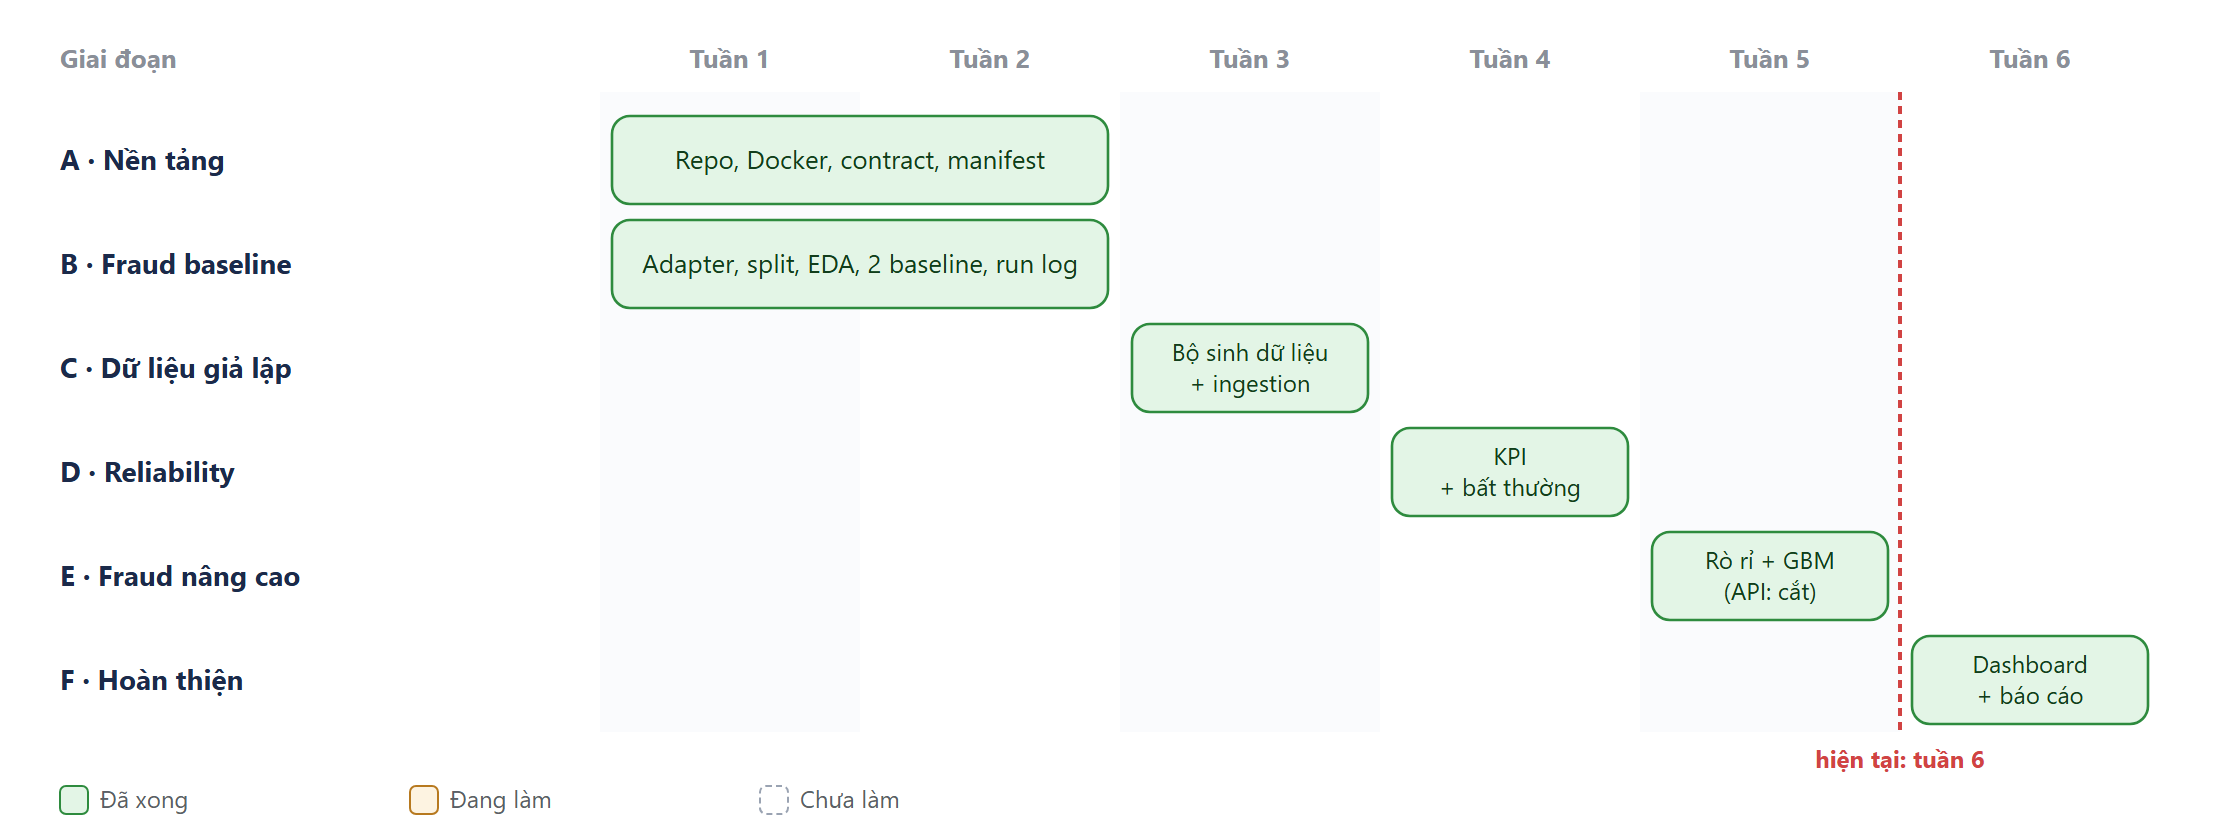
\includegraphics[width=0.95\linewidth]{figures/roadmap.png}
\caption{Lộ trình 6 tuần theo giai đoạn A--F.}
\end{figure}

% ================================================================ 2
\section{Kiến trúc hệ thống}

\begin{figure}[H]\centering
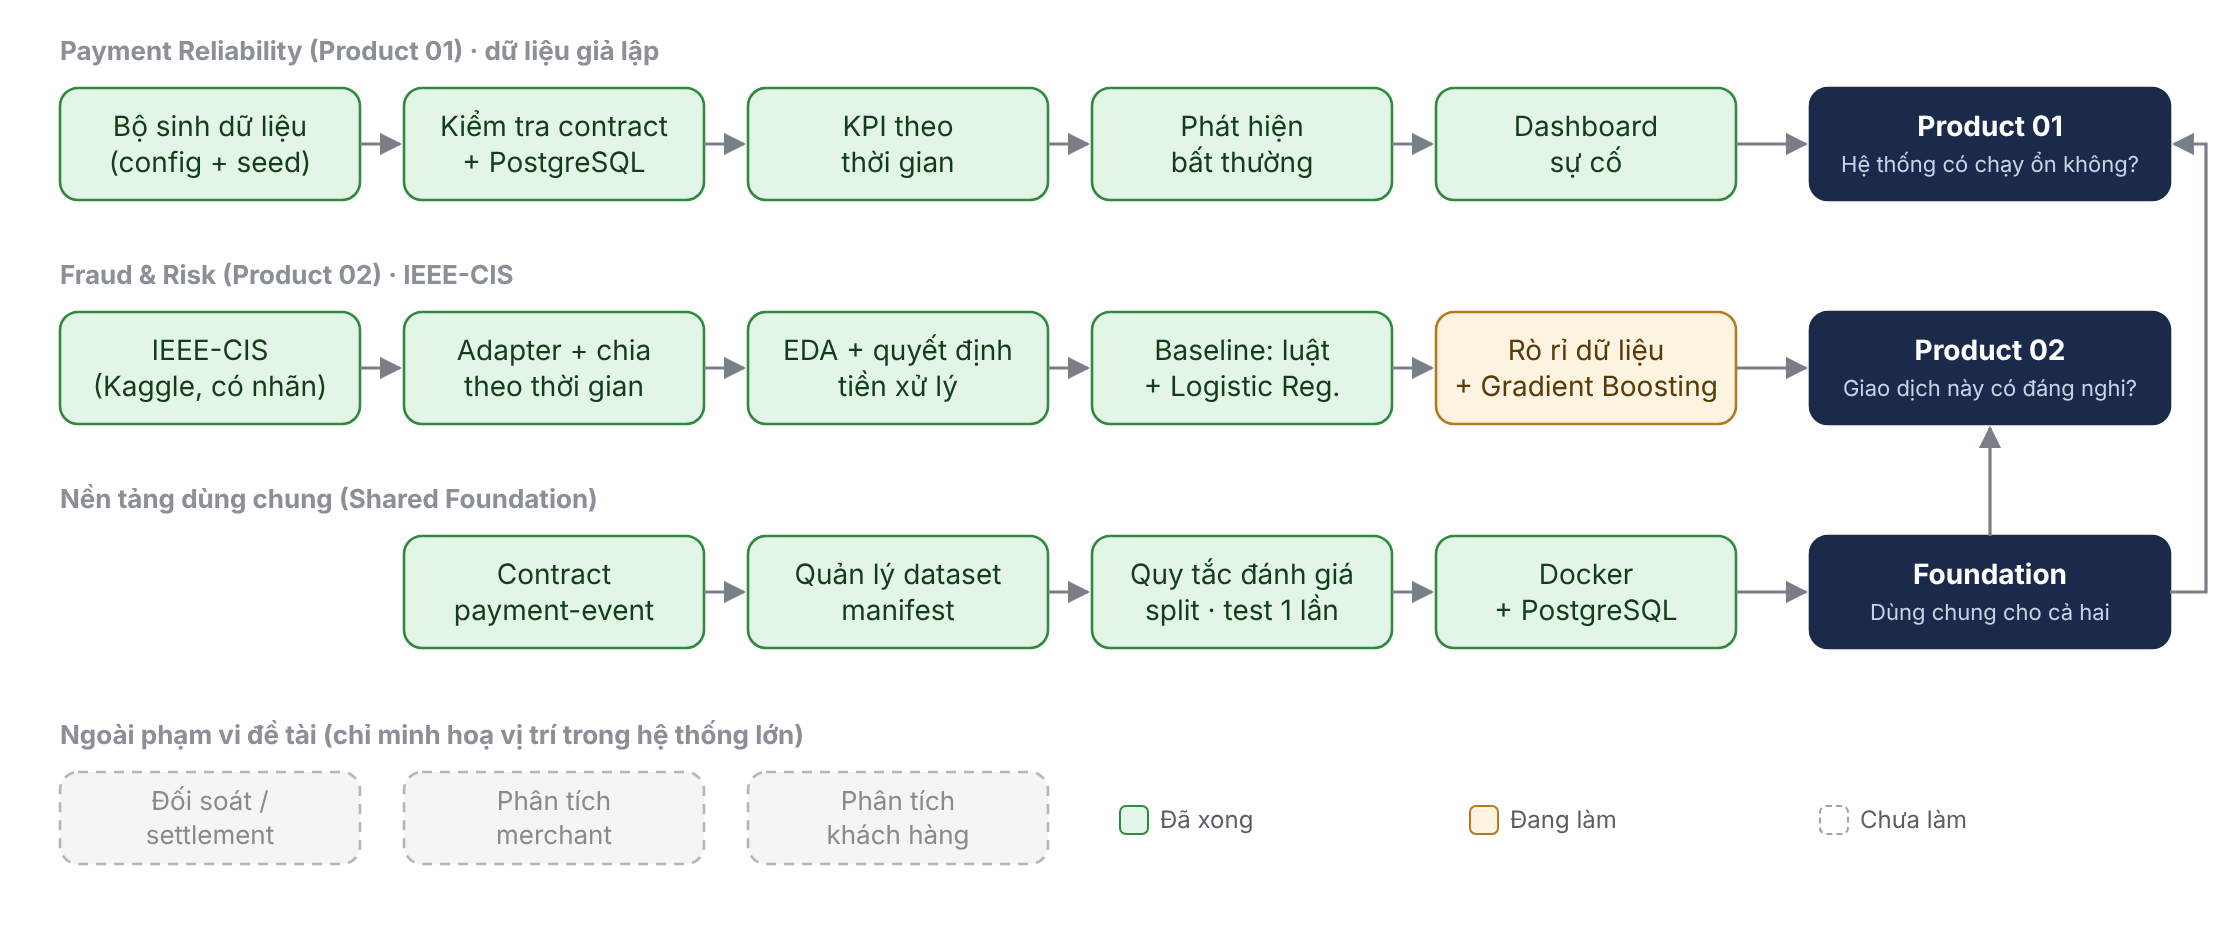
\includegraphics[width=\linewidth]{figures/system-overview.png}
\caption{Nền tảng dùng chung và hai sản phẩm. Hai sản phẩm dùng chung công cụ nhưng không dùng chung dữ liệu (ADR 0002).}
\end{figure}

\begin{tabularx}{\linewidth}{@{}lX@{}}
\toprule
\textbf{Thành phần} & \textbf{Vai trò} \\ \midrule
Contract \code{payment-event} 1.0.0 & JSON Schema mô tả một sự kiện thanh toán; mọi dữ liệu Product 01 phải qua kiểm tra này \\
Quản lý dataset & Manifest YAML ghi nguồn, giấy phép và checksum SHA-256 của từng file dữ liệu \\
Quy tắc đánh giá & Chia theo thời gian, test một lần, mã lần chạy tất định (mục 3.6) \\
PostgreSQL 16 & Lưu sự kiện Product 01; KPI tính bằng SQL views (ADR 0005) \\
Dashboard & Trang HTML tĩnh tổng hợp kết quả hai sản phẩm (ADR 0007) \\ \bottomrule
\end{tabularx}

% ================================================================ 3
\section{Kiến thức nền tảng}

\subsection{Dữ liệu mất cân bằng và cách đo mô hình}

Trong IEEE-CIS chỉ khoảng 3,5\% giao dịch là gian lận. Một mô hình luôn đoán ``không gian lận'' đạt độ chính xác (accuracy) 96,5\% nhưng vô dụng. Vì vậy đề tài \textbf{không} dùng accuracy làm chỉ số chính.

Với một ngưỡng quyết định, mỗi giao dịch rơi vào một trong bốn ô: TP (gian lận, báo đúng), FP (hợp lệ, báo nhầm), FN (gian lận, bỏ sót), TN (hợp lệ, không báo).
\[
\text{Precision}=\frac{TP}{TP+FP},\qquad
\text{Recall}=\frac{TP}{TP+FN},\qquad
\text{FPR}=\frac{FP}{FP+TN},\qquad
F_1=\frac{2\,PR}{P+R}.
\]
\begin{itemize}
  \item \textbf{Precision}: trong các cảnh báo, bao nhiêu phần trăm đúng. \textbf{Recall}: trong các giao dịch gian lận, bắt được bao nhiêu.
  \item \textbf{PR-AUC} (average precision): diện tích dưới đường precision--recall khi quét mọi ngưỡng, $\text{AP}=\sum_n (R_n-R_{n-1})P_n$. Mô hình ngẫu nhiên có PR-AUC bằng \emph{tỷ lệ gian lận}, nên PR-AUC 0,165 trên tập có 3,44\% gian lận nghĩa là gấp khoảng 4,8 lần ngẫu nhiên. Trên dữ liệu mất cân bằng, đường PR cho nhiều thông tin hơn đường ROC \cite{saito}.
\end{itemize}

\begin{explain}{Recall tại FPR cố định}
Precision phụ thuộc vào tỷ lệ gian lận: cùng một mô hình, tập nào nhiều gian lận hơn thì precision cao hơn. Vì validation (3,90\%) và test (3,44\%) có tỷ lệ khác nhau, so precision giữa hai tập dễ hiểu nhầm.

FPR chỉ tính trên giao dịch hợp lệ nên \emph{không} phụ thuộc tỷ lệ gian lận. Chỉ số ``recall tại FPR 5\%'' trả lời câu hỏi vận hành: \emph{nếu chỉ chấp nhận làm phiền 5\% khách hàng hợp lệ, ta bắt được bao nhiêu phần trăm gian lận?} Cách tính: quét các ngưỡng từ cao xuống thấp, giữ các ngưỡng có FPR $\le 5\%$, lấy recall lớn nhất. Chỉ số này được khuyến nghị cho dữ liệu gian lận có thay đổi theo thời gian \cite{jesus}. Mô hình ngẫu nhiên đạt đúng 0,05.
\end{explain}

\begin{explain}{Khoảng tin cậy bootstrap cho PR-AUC}
Một con số PR-AUC tính trên khoảng 118 nghìn dòng vẫn có sai số do chọn mẫu. Bootstrap ước lượng sai số đó mà không cần công thức:
\begin{enumerate}
  \item Lấy ngẫu nhiên \emph{có hoàn lại} $n$ dòng từ $n$ dòng của tập đánh giá (có dòng lặp, có dòng vắng).
  \item Tính PR-AUC trên mẫu đó. Lặp lại $B=200$ lần, với seed cố định để tái lập.
  \item Khoảng tin cậy 95\% là phân vị 2,5\% và 97,5\% của 200 giá trị.
\end{enumerate}
Ví dụ: Logistic Regression trên test có PR-AUC 0,165 [0,155; 0,176]. Hai mô hình có khoảng tin cậy không chồng nhau thì khác biệt khó là do may rủi.
\end{explain}

\subsection{Chia dữ liệu theo thời gian và rò rỉ dữ liệu}

\textbf{Chia theo thời gian.} Mô hình dùng thật luôn chấm điểm giao dịch \emph{trong tương lai}. Vì vậy dữ liệu được xếp theo thời gian rồi chia 60\% đầu làm train, 20\% tiếp theo làm validation, 20\% cuối làm test. Chia ngẫu nhiên sẽ cho mô hình ``nhìn thấy tương lai'' và làm kết quả lạc quan giả tạo. Hành vi gian lận thay đổi theo thời gian (\emph{concept drift} \cite{gama}), nên điểm trên test thường thấp hơn trên validation; đề tài quan sát đúng điều này (mục 4).

\textbf{Vai trò ba tập.} Train để học. Validation để chọn ngưỡng và siêu tham số. Test để đo một lần cuối. Nếu nhìn kết quả test rồi chỉnh mô hình, test trở thành một tập validation thứ hai và mất giá trị.

\textbf{Rò rỉ dữ liệu} (data leakage) là khi mô hình dùng thông tin không có tại thời điểm dự đoán thật \cite{kaufman}. Các kiểu thường gặp \cite{kapoor}:
\begin{itemize}
  \item \emph{Không tách train/test đúng cách}: chia ngẫu nhiên với dữ liệu có thời gian; fit tiền xử lý (chuẩn hoá, điền thiếu) trên toàn bộ dữ liệu.
  \item \emph{Đặc trưng mang nhãn}: một cột được tính từ nhãn của chính tập đánh giá.
  \item \emph{Thông tin tương lai}: đặc trưng chỉ có sau thời điểm giao dịch.
\end{itemize}

\begin{explain}{Quy tắc test một lần và sổ đăng ký}
Mỗi cấu hình có trường \code{status: draft} hoặc \code{frozen}. Lệnh chạy test (\code{make baseline-final}, \code{make gbm-final}, \code{make detect-report}) từ chối cấu hình chưa \code{frozen}. Khi chạy, nó tính một mã băm (hash) từ cấu hình và ghi vào sổ đăng ký (\code{artifacts/test\_runs.json}). Lần chạy thứ hai với cùng hash bị từ chối, trừ khi dùng \code{--force}; khi đó cảnh báo được ghi thẳng vào kết quả. Muốn thử mô hình khác sau khi xem test thì phải tạo cấu hình mới, và báo cáo phải nói rõ.

Danh sách cấu hình được phép chạy test được \emph{đăng ký trước} trong đặc tả. Ở Stage E chỉ có một: Gradient Boosting không có khoảng trống thời gian.
\end{explain}

\begin{explain}{Độ trễ nhãn và khoảng trống thời gian (\code{gap\_days})}
Trong thực tế, nhãn gian lận đến muộn: chargeback có thể mất vài tuần. Trong IEEE-CIS nhãn đã có sẵn, và theo mô tả của ban tổ chức, nhãn còn lan sang các giao dịch sau của cùng tài khoản. Nếu train kết thúc sát ngày validation bắt đầu, mô hình biết nhãn của cả những giao dịch mà ngoài đời chưa có nhãn.

Đề tài mô phỏng điều này bằng cách bỏ $N$ ngày cuối của train ($N=7$, $14$) và giữ nguyên validation, test. Vì tập đánh giá không đổi, mọi khác biệt chỉ do khoảng trống. Đây là \emph{phân tích độ nhạy}, không phải ``giá trị đúng'' (ADR 0003).
\end{explain}

\subsection{Logistic Regression}
Mô hình tính xác suất gian lận
\[
p(x)=\sigma(w^\top x+b),\qquad \sigma(z)=\frac{1}{1+e^{-z}},
\]
và học $w,b$ bằng cách tối thiểu hoá log-loss có trọng số:
\[
L=-\sum_i c_{y_i}\bigl[y_i\log p(x_i)+(1-y_i)\log(1-p(x_i))\bigr].
\]
Với \code{class\_weight='balanced'}, trọng số mỗi lớp là $c_k=\dfrac{n}{2\,n_k}$. Trên train: $c_1\approx 14{,}78$ cho gian lận và $c_0\approx 0{,}52$ cho hợp lệ, nên mô hình không bỏ qua lớp hiếm. Trước khi vào mô hình, cột số được điền thiếu bằng trung vị và chuẩn hoá $(x-\mu)/\sigma$; cột phân loại được one-hot. Cả trung vị, $\mu$, $\sigma$ và danh mục đều chỉ học trên train, trong một \code{Pipeline} của scikit-learn.

\subsection{Gradient Boosting}
Gradient Boosting cộng dần nhiều cây quyết định nhỏ:
\[
F_m(x)=F_{m-1}(x)+\nu\,h_m(x),
\]
trong đó mỗi cây $h_m$ được học để sửa sai của các cây trước (khớp với gradient âm của log-loss), và $\nu$ là tốc độ học (0,05 hoặc 0,1). Mô hình cây thường mạnh trên dữ liệu bảng \cite{grinsztajn}, không cần chuẩn hoá, và tự xử lý giá trị thiếu.

\code{HistGradientBoostingClassifier} của scikit-learn chia giá trị mỗi cột thành tối đa 255 ``thùng'' (histogram) trước khi tìm điểm chia, nên nhanh trên vài trăm nghìn dòng. Đề tài tắt \code{early\_stopping} vì phần validation nội bộ của nó chia \emph{ngẫu nhiên}, trái quy tắc chia theo thời gian. Số cây (\code{max\_iter}) nằm trong lưới 8 tổ hợp, chọn theo PR-AUC trên validation (ADR 0006).

\subsection{Mã hoá theo nhãn (target encoding)}
Cột \code{card1} (định danh thẻ) có hơn 10 nghìn giá trị, không one-hot được. Mã hoá theo nhãn thay mỗi giá trị $v$ bằng tỷ lệ gian lận đã làm mượt:
\[
\text{enc}(v)=\frac{\sum_{i:\,x_i=v}y_i+m\cdot\bar{y}}{n_v+m},
\]
với $\bar y$ là tỷ lệ gian lận chung và $m=100$ kéo các giá trị hiếm về $\bar y$.

\begin{explain}{Mã hoá ngoài fold (out-of-fold) và vì sao cần}
Nếu mã hoá một dòng train bằng tỷ lệ gian lận có tính cả nhãn của \emph{chính dòng đó}, đặc trưng ``biết trước'' đáp án trên train. Mô hình học cách tin vào đặc trưng này quá mức, rồi thất vọng trên validation. Trên dữ liệu thử nghiệm, cách làm này làm PR-AUC \emph{giảm} từ 0,168 xuống 0,078.

Cách sửa: chia train thành 5 khối liên tiếp theo thời gian; mỗi khối được mã hoá bằng nhãn của 4 khối còn lại. Validation và test được mã hoá bằng nhãn của toàn bộ train. Khi đó không dòng nào dùng nhãn của chính nó, và PR-AUC trên dữ liệu thử về lại 0,166. Thí nghiệm rò rỉ (mục 4.3) so sánh bản này với bản cố tình dùng cả nhãn validation.
\end{explain}

\subsection{Tái lập kết quả}

\begin{explain}{Mã lần chạy tất định (run id)}
Mỗi lần chạy có mã \code{run-} + 12 ký tự đầu của SHA-256 tính trên: cấu hình dạng chuẩn hoá (bỏ trường \code{status}), seed, checksum của dataset và mốc chia dữ liệu. Cùng điều kiện thì cùng mã và cùng kết quả (có kiểm thử so từng byte của \code{metrics.json}). Đổi bất kỳ yếu tố nào thì ra mã mới. Mã git commit \emph{không} nằm trong hash, vì sửa tài liệu không làm thay đổi một lần chạy. Bộ sinh dữ liệu dùng cùng ý tưởng cho \code{simulation\_id}.
\end{explain}

\subsection{Mô phỏng dữ liệu thanh toán}
\begin{itemize}
  \item \textbf{Số giao dịch mỗi giờ} theo phân phối Poisson với cường độ $\lambda_h=150\times f_{\text{giờ}}\times f_{\text{ngày}}$; hệ số theo giờ Việt Nam (thấp ban đêm, cao buổi trưa và tối), trung bình bằng 1.
  \item \textbf{Số tiền và độ trễ} theo phân phối log-normal (lệch phải, luôn dương), tham số theo phương thức thanh toán và theo provider.
  \item \textbf{Lỗi và retry}: mỗi provider có xác suất lỗi riêng (15\%, 22\%, 30\%, cố ý để cao). Chỉ lỗi kỹ thuật (\code{TIMEOUT}, \code{PROVIDER\_ERROR}, \code{NETWORK\_ERROR}) được thử lại; lỗi nghiệp vụ (\code{DECLINED}, \code{INVALID\_REQUEST}) thì không.
  \item \textbf{Sự cố cài sẵn}: provider lỗi, độ trễ tăng, bùng lỗi mạng, mất lưu lượng một phương thức; mỗi loại có độ lớn (ví dụ x3 nghĩa là xác suất lỗi nhân 3). Nhãn sự cố chỉ nằm trong \code{anomaly\_labels.json}, không có trong sự kiện.
\end{itemize}

\begin{explain}{Luồng số ngẫu nhiên riêng cho từng payment}
Mỗi payment dùng một bộ sinh số ngẫu nhiên riêng, khởi tạo từ (seed, số thứ tự payment). Nhờ vậy, khi cài thêm một sự cố trong một cửa sổ thời gian, chỉ các payment chạm vào cửa sổ đó thay đổi; mọi payment khác giống hệt lần chạy không có sự cố. Kiểm thử xác nhận hơn 90\% payment không đổi. Điều này cho phép so sánh ``có sự cố'' và ``không có sự cố'' trên \emph{cùng} một thế giới giả lập.
\end{explain}

\subsection{Phát hiện bất thường trên chuỗi KPI}

KPI được tính cho từng khung 15 phút và từng provider: tỷ lệ lỗi kỹ thuật, trung vị độ trễ, và tỷ trọng mỗi phương thức trong các payment mới. Ba KPI này ứng với ba trong bốn ``tín hiệu vàng'' của giám sát hệ thống (errors, latency, traffic) \cite{sre}.

\begin{explain}{z-score bền vững (detector D-A, đường cơ sở)}
z-score thông thường $(x-\mu)/\sigma$ bị kéo lệch khi trong lịch sử có vài giá trị cực đoan. Bản bền vững thay trung bình bằng \emph{trung vị} và độ lệch chuẩn bằng \emph{MAD} (trung vị của độ lệch tuyệt đối):
\[
z_t=\frac{x_t-\operatorname{median}(x_{t-96..t-1})}{1{,}4826\cdot\operatorname{MAD}(x_{t-96..t-1})}.
\]
Hệ số 1,4826 làm MAD bằng độ lệch chuẩn khi dữ liệu có phân phối chuẩn. Lịch sử là 96 khung trước đó (24 giờ).

\textbf{Điểm yếu:} D-A không biết một tỷ lệ được tính trên bao nhiêu attempt. Ban đêm một khung chỉ có vài attempt, một lỗi trên hai attempt thành 50\% và cho điểm rất cao. Kết quả thực nghiệm đúng như vậy: 14 lần báo nhầm của D-A đều rơi vào 01:45--05:45 giờ Việt Nam.
\end{explain}

\begin{explain}{Điểm nhị thức gộp cửa sổ (detector D-B, phương án chính)}
Ý tưởng: thay vì so \emph{tỷ lệ}, so \emph{số lỗi quan sát được} với số lỗi kỳ vọng, có tính đến số attempt.
\begin{enumerate}
  \item Gộp $k=2$ khung gần nhất (30 phút): có $N$ attempt và $K$ lỗi.
  \item Lấy tỷ lệ lỗi nền $p_0$ từ 24 giờ trước cửa sổ đó.
  \item Nếu không có sự cố, $K$ xấp xỉ phân phối nhị thức $\mathrm{Bin}(N,p_0)$, có trung bình $Np_0$ và độ lệch chuẩn $\sqrt{Np_0(1-p_0)}$. Điểm là số độ lệch chuẩn vượt kỳ vọng:
  \[
  z=\frac{K-Np_0}{\sqrt{Np_0(1-p_0)}}.
  \]
\end{enumerate}
Với cùng một mức tăng tỷ lệ, $N$ nhỏ (ban đêm) cho $z$ nhỏ, $N$ lớn cho $z$ lớn: detector tự ``bớt tin'' các khung ít dữ liệu. Với tỷ trọng phương thức (sự cố mất lưu lượng), $K$ là số payment mới của phương thức đó, $N$ là tổng payment mới; điểm được đổi dấu vì bất thường là \emph{giảm}. Với độ trễ, D-B lấy trung bình log-trung vị có trọng số theo số attempt và chia cho độ phân tán đã chuẩn hoá theo $\sqrt{n}$.

\textbf{Vì sao ngưỡng phải cao (8 thay vì 3).} Có 12 chuỗi KPI, mỗi chuỗi 672 khung trong 7 ngày, tức khoảng 8 nghìn lần kiểm tra. Ngưỡng 3 độ lệch chuẩn, nếu xét riêng từng lần, chỉ sai khoảng 0,13\%, nhưng nhân với 8 nghìn lần là khoảng 10 lần báo nhầm trong 7 ngày. Lưới chỉnh ngưỡng xác nhận đúng như vậy: ngưỡng 3 báo nhầm 1,4--1,9 lần mỗi ngày, ngưỡng 8 không báo nhầm lần nào. Đây là vấn đề \emph{kiểm định nhiều lần} (multiple testing).
\end{explain}

\textbf{Đánh giá theo sự cố.} Các khung cảnh báo liền nhau (cách nhau tối đa 1 khung) được gộp thành một \emph{sự cố}. Một bất thường cài sẵn được tính là ``bắt được'' nếu có sự cố \emph{đúng đối tượng} (đúng provider, hoặc đúng phương thức) giao với cửa sổ của nó (cộng 15 phút ân hạn). Chỉ số báo cáo: số bất thường bắt được, độ trễ phát hiện, số sự cố báo nhầm mỗi ngày. Cách chấm theo cửa sổ dựa trên \cite{lavin}; rủi ro ``bất thường quá dễ'' theo \cite{wu}.

\begin{explain}{Tách bộ dữ liệu chỉnh ngưỡng và bộ báo cáo}
Nếu chỉnh ngưỡng và đo kết quả trên cùng một bộ dữ liệu giả lập, ta chỉ chứng minh được rằng detector khớp với bộ đó. Vì vậy có hai bộ: \emph{tuning} (seed 42) để chỉnh ngưỡng, và \emph{report} (seed 2026) để đo một lần, có một loại sự cố mà bộ tuning không có (mất lưu lượng). Đây là phiên bản ``train/test'' cho bài toán không có nhãn thật.
\end{explain}

\subsection{Kỹ thuật dữ liệu}
\begin{itemize}
  \item \textbf{Data contract} bằng JSON Schema \cite{jsonschema}: quy định trường, kiểu, giá trị cho phép; cấm trường lạ (ví dụ \code{card\_number}). Quy tắc mà schema không diễn đạt được (ví dụ \code{payment\_id} khác \code{attempt\_id}, các attempt của một payment phải cùng số tiền) được kiểm tra bằng code.
  \item \textbf{Ingestion idempotent}: nạp lại cùng file không tạo bản ghi trùng (khoá chính \code{event\_id} và \code{INSERT … ON CONFLICT DO NOTHING}); file đã đổi nội dung thì bị từ chối. Thử nghiệm: nạp lại 30.050 sự kiện, thêm 0 dòng.
  \item \textbf{SQL views}: KPI là các câu SQL đọc được trực tiếp (\code{date\_bin} để chia khung 15 phút, \code{percentile\_cont} cho phân vị, \code{generate\_series} để giữ cả khung trống). Kiểm thử so kết quả view với một cách tính độc lập bằng pandas.
\end{itemize}

\subsection{Đặc trưng lịch sử thực thể và so sánh hai mô hình}

\begin{explain}{Đặc trưng lịch sử chỉ nhìn quá khứ}
Một \emph{thực thể} là nhóm giao dịch có vẻ cùng một khách hàng. Đề tài thử ba khoá: \code{card1} (định danh thẻ, khoảng 13,6 nghìn giá trị nên trộn nhiều khách hàng); \code{card1}+\code{addr1}+\code{P\_emaildomain} (gọi là \emph{uid}); và uid thêm \code{D1n} = ngày giao dịch trừ \code{D1}. \code{D1} là số ngày kể từ khi thẻ bắt đầu dùng, nên \code{D1n} gần như không đổi với một thẻ và tách được các khách hàng dùng chung uid. Ý tưởng các khoá này lấy từ thảo luận công khai của cuộc thi.

Với mỗi giao dịch, đặc trưng chỉ dùng các giao dịch \emph{trước đó} của cùng thực thể, không dùng nhãn: số giao dịch trong 24 giờ và 7 ngày trước; số tiền chia trung bình số tiền trước; số giây từ giao dịch trước; độ lệch chuẩn và z-score của số tiền; số giá trị \code{ProductCD} và \code{C13} khác nhau đã gặp. Giao dịch cùng giây thấy giao dịch đứng trước trong file nhưng không thấy giao dịch đứng sau. Kiểm thử xác nhận: đổi một giao dịch sau không làm đổi đặc trưng của bất kỳ giao dịch nào trước nó.

Các bài viết công khai của cuộc thi gộp thống kê trên \emph{toàn bộ} dữ liệu, tức là có cả giao dịch tương lai và tập đánh giá. Hệ thống thật không có thông tin đó, nên đề tài chỉ lấy ý tưởng và tính lại theo quá khứ.
\end{explain}

\begin{explain}{Bootstrap cặp và bootstrap theo cụm}
Hai mô hình có khoảng tin cậy chồng nhau chưa chắc là ngang nhau: phần lớn sai số đến từ việc \emph{cùng} một tập đánh giá có dòng dễ, dòng khó, và sai số đó chung cho cả hai. \textbf{Bootstrap cặp} lấy mẫu lại các dòng một lần rồi tính PR-AUC của \emph{cả hai} mô hình trên cùng mẫu đó và lấy hiệu; lặp 500 lần, khoảng tin cậy của hiệu hẹp hơn nhiều so với so hai khoảng riêng.

Lấy mẫu theo dòng giả định các dòng độc lập. Nhưng giao dịch của cùng một thẻ giống nhau, nên giả định này làm khoảng tin cậy \emph{quá hẹp}. \textbf{Bootstrap theo cụm} lấy mẫu lại cả nhóm \code{card1} (mọi giao dịch của một thẻ đi cùng nhau). Trên IEEE-CIS, khoảng theo cụm rộng gấp khoảng hai lần khoảng theo dòng, và đây là con số đề tài dùng để kết luận.

Trước khi so, mỗi mô hình được huấn luyện lại với đúng tham số đã chọn; PR-AUC validation phải khớp số đã ghi trong lần chạy, nếu không chương trình dừng với lỗi.
\end{explain}

% ================================================================ 4
\section{Product 02 — Rủi ro gian lận trên IEEE-CIS}

\subsection{Dữ liệu và phân tích khám phá}
590.540 giao dịch trong khoảng 6 tháng. Chia theo thời gian:

\begin{figure}[H]\centering
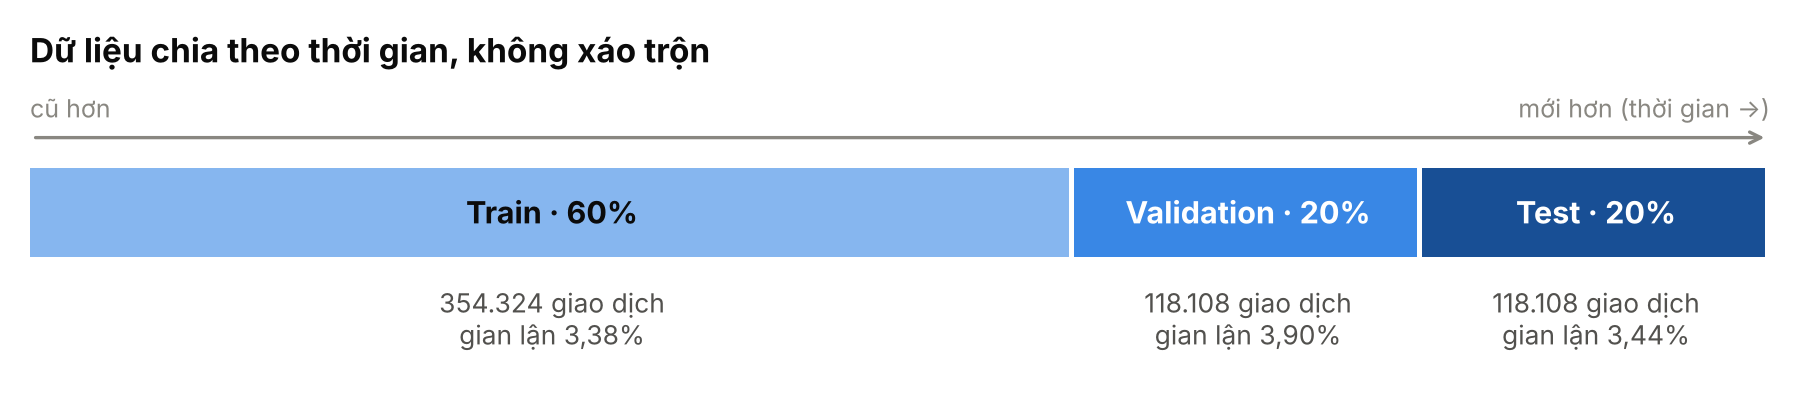
\includegraphics[width=0.9\linewidth]{figures/split.png}
\caption{Chia dữ liệu theo thời gian, không xáo trộn.}
\end{figure}

Phân tích khám phá (EDA) chỉ chạy trên train và cho ra 9 quyết định tiền xử lý, mỗi quyết định có bằng chứng và được chủ dự án duyệt (\code{docs/data-analysis/eda-summary.md}). Ví dụ:
\begin{itemize}
  \item \code{TransactionAmt} lệch phải rất mạnh (độ lệch 19,44; trung vị 70, lớn nhất 31.937), nên thêm $\log(1+x)$ (độ lệch còn 0,50).
  \item Fraud rate theo tuần trên train dao động 1,85\%--4,55\%, nên dùng \code{class\_weight='balanced'} và chọn ngưỡng trên validation.
  \item Loại \code{TransactionID} và \code{TransactionDT} gốc vì chúng mã hoá thứ tự thời gian; chỉ dùng giờ trong ngày.
\end{itemize}

\subsection{Hai baseline (Stage B)}
Baseline luật: 3 luật minh bạch có ngưỡng học trên train (số tiền trên phân vị 99; \code{ProductCD} và loại thẻ có tỷ lệ gian lận cao); điểm là tỷ lệ luật bị kích hoạt. Logistic Regression: 20 đặc trưng (số tiền, log số tiền, giờ trong ngày, 14 cột đếm \code{C1}--\code{C14}, \code{ProductCD}, \code{card4}, \code{card6}).

\begin{table}[H]\centering
\caption{Kết quả lần chạy \code{run-d6faa4699008}, cấu hình đã \code{frozen}. Tập test mở một lần.}
\begin{tabular}{@{}llccc@{}}
\toprule
Mô hình & Tập & PR-AUC [95\% CI] & Tỷ lệ gian lận & Recall @ FPR 5\% \\ \midrule
Logistic Regression & Validation & 0,245 [0,234; 0,256] & 3,90\% & 0,33 \\
Logistic Regression & \textbf{Test} & \textbf{0,165} [0,155; 0,176] & 3,44\% & 0,28 \\
Luật & Validation & 0,089 [0,084; 0,092] & 3,90\% & 0,00 \\
Luật & \textbf{Test} & \textbf{0,078} [0,074; 0,082] & 3,44\% & 0,22 \\ \bottomrule
\end{tabular}
\end{table}

\begin{figure}[H]\centering
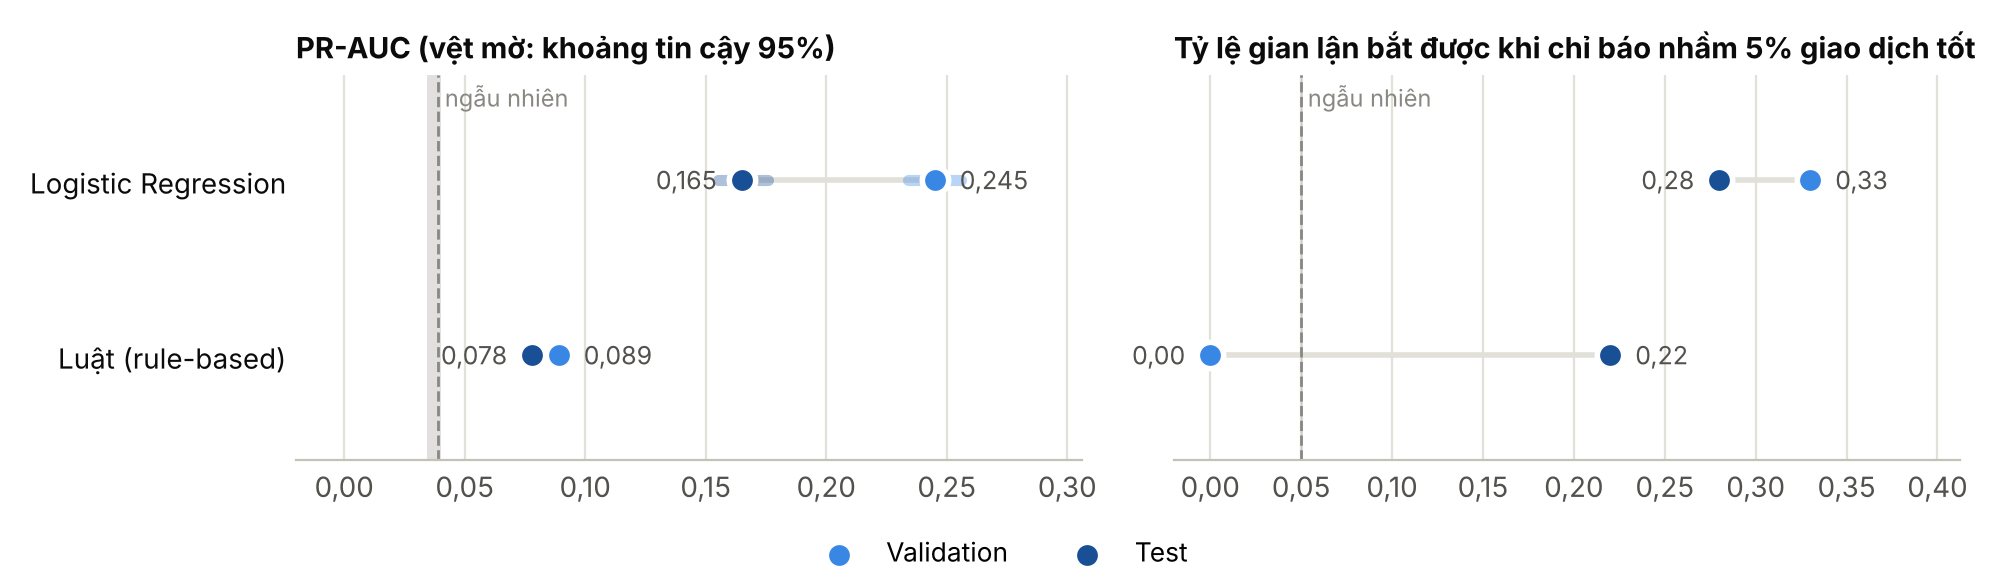
\includegraphics[width=\linewidth]{figures/results.png}
\caption{Validation (nhạt) và test (đậm) của hai mô hình. Vùng xám: mức của mô hình ngẫu nhiên.}
\end{figure}

\begin{keypoint}
\textbf{Đọc kết quả.} (1) Logistic Regression tốt hơn luật rõ rệt; khoảng tin cậy không chồng nhau. (2) Kết quả giảm từ validation sang test, kể cả chỉ số không phụ thuộc tỷ lệ gian lận (recall tại FPR 5\%: 0,33 → 0,28), nên mức giảm không chỉ do tỷ lệ gian lận thấp hơn: dữ liệu thay đổi theo thời gian. (3) Số 0 của baseline luật trên validation là do điểm luật chỉ có vài mức rời rạc: mức chặt nhất báo nhầm 5,1\% giao dịch tốt, vượt mục tiêu 5\% một chút. (4) Có hai lần chạy test (\code{run-515a1190a0a4} trước khi thêm chỉ số FPR, và \code{run-d6faa4699008}); mọi chỉ số chung trùng khớp, nên lần thứ hai không dùng để chọn lại mô hình.
\end{keypoint}

\subsection{Thí nghiệm rò rỉ dữ liệu (Stage E)}
Lấy đúng Logistic Regression của Stage B, mỗi biến thể phá \emph{một} quy tắc, tất cả đo trên validation:

\begin{tabularx}{\linewidth}{@{}lX@{}}
\toprule
Biến thể & Thay đổi \\ \midrule
Đúng quy tắc & Như Stage B (mốc so sánh) \\
Chia ngẫu nhiên & Xáo trộn trước khi chia 60/20/20 \\
Tiền xử lý trên mọi dòng & Điền thiếu, chuẩn hoá, one-hot fit trên toàn bộ dữ liệu \\
Mã hoá \code{card1} hợp lệ & Thêm mã hoá theo nhãn, ngoài fold trên train \\
Mã hoá \code{card1} rò rỉ & Mã hoá bằng nhãn train \emph{và validation} \\
Khoảng trống 7, 14 ngày & Bỏ cuối train (độ trễ nhãn) \\ \bottomrule
\end{tabularx}

Kèm bảng mô tả \emph{thực thể lặp lại}: bao nhiêu phần trăm dòng validation và test có thẻ (\code{card1}, và tổ hợp \code{card1}+\code{addr1}+\code{P\_emaildomain}) đã xuất hiện trong train. Tổ hợp ba cột là kinh nghiệm phổ biến trong các notebook công khai của cuộc thi; đề tài chỉ dùng ý tưởng, không sao chép code.

\begin{table}[H]\centering
\caption{Lần chạy \code{leak-827d929eaa73}, chỉ trên validation (118.108 dòng). Không đọc nhãn test.}
\begin{tabular}{@{}lccc@{}}
\toprule
Biến thể & PR-AUC [95\% CI] & Chênh & Recall @ FPR 5\% \\ \midrule
Đúng quy tắc (Stage B) & 0,245 [0,235; 0,257] & +0,000 & 0,33 \\
Chia ngẫu nhiên & 0,177 [0,168; 0,190] & $-$0,068 & 0,31 \\
Tiền xử lý trên mọi dòng & 0,244 [0,234; 0,256] & $-$0,001 & 0,33 \\
Mã hoá \code{card1} hợp lệ & 0,252 [0,242; 0,264] & +0,007 & 0,37 \\
Mã hoá \code{card1} rò rỉ & 0,308 [0,297; 0,321] & \textbf{+0,063} & 0,43 \\
Khoảng trống 7 ngày & 0,244 [0,233; 0,256] & $-$0,002 & 0,32 \\
Khoảng trống 14 ngày & 0,241 [0,231; 0,253] & $-$0,004 & 0,32 \\ \bottomrule
\end{tabular}
\end{table}

Thực thể lặp lại: 98,7\% dòng validation có \code{card1} đã gặp trong train; với \code{card1}+\code{addr1}+\code{P\_emaildomain} là 85,9\%.

\begin{keypoint}
\textbf{Đọc kết quả.} (1) Rò nhãn rõ nhất là mã hoá \code{card1} bằng nhãn validation: PR-AUC tăng 0,063, trong khi bản dùng nhãn train đúng cách chỉ tăng 0,007. (2) Tiền xử lý trên mọi dòng và khoảng trống 7--14 ngày đổi PR-AUC không quá 0,004, nhỏ hơn độ rộng khoảng tin cậy (khoảng 0,02): với baseline này chúng không tạo khác biệt đo được. (3) \textbf{Ngược kỳ vọng}, chia ngẫu nhiên cho PR-AUC \emph{thấp hơn} 0,068. Chẩn đoán bên dưới cho thấy nguyên nhân chủ yếu nằm ở tập đánh giá, không ở mô hình.
\end{keypoint}

\begin{keypoint}
\textbf{Chẩn đoán chia ngẫu nhiên} (lần chạy \code{diag-827d929eaa73}, chỉ train và validation, không đụng test). (1) Ma trận 2$\times$2: đổi cách huấn luyện chỉ đổi PR-AUC 0,001--0,012, đổi tập đánh giá đổi khoảng 0,07; các validation là hai tập dòng khác nhau. (2) Tỷ lệ gian lận chỉ giải thích khoảng 0,012. (3) Validation ngẫu nhiên có tuần 0--3 (khoảng 31.000 dòng) với tỷ lệ gian lận 1,9--2,8\% và PR-AUC thấp; bỏ các tuần này thì PR-AUC tăng từ 0,179 lên 0,212, giải thích khoảng một nửa mức chênh. Việc chọn tuần 0--3 được quyết định \emph{sau} khi xem bảng theo tuần. (4) Còn khoảng 0,03 chưa giải thích. (5) Recall tại FPR 5\% gần như không đổi (0,31--0,34): không có bằng chứng chia ngẫu nhiên làm \emph{mô hình} kém đi. Trên cùng 29.223 dòng, mô hình huấn luyện ngẫu nhiên hơn +0,0117 [0,0087; 0,0145] (khoảng này hẹp hơn thực tế vì lấy mẫu theo dòng).
\end{keypoint}

\begin{keypoint}
\textbf{Đặc trưng lịch sử thực thể} (chỉ validation, mọi config ở trạng thái nháp). (1) Đếm tích luỹ không dừng theo thời gian (số giữa \code{card1} 186 ở train, 629 ở validation), nhưng đếm theo cửa sổ 24 giờ và 7 ngày cũng không giúp. (2) Bỏ \code{C1}--\code{C14} thì PR-AUC validation rơi từ 0,497 xuống 0,158: các cột này mang gần như toàn bộ tín hiệu theo thực thể, mạnh hơn lịch sử tự dựng (thêm lịch sử chỉ nâng lên 0,174--0,177). Việc các cột này đếm gì lấy từ thảo luận công khai, chưa xác minh. (3) Lưới \code{max\_iter} đến 1.200 không tốt hơn 400. (4) Khoá có \code{D1n} cho +0,0114 PR-AUC khi lấy mẫu theo dòng, nhưng [$-$0,0026; +0,0249] khi lấy mẫu theo cụm \code{card1}, chỉ recall tại FPR 5\% (+0,0218 [+0,0033; +0,0424]) loại trừ 0; chưa hiệu chỉnh nhiều lần so sánh. (5) Áp ý tưởng thống kê tổng hợp theo thực thể của các giải pháp công khai (độ lệch chuẩn, z-score của số tiền, số giá trị khác nhau của \code{ProductCD} và \code{C13}), nhưng chỉ dùng giao dịch \emph{trước đó}: PR-AUC 0,4968 và 0,4984, chênh so với gốc theo cụm \code{card1} là $-$0,0002 [$-$0,0094; +0,0093] và +0,0022 [$-$0,0117; +0,0173]; không giúp. Theo nguồn thứ cấp, họ gộp trên toàn bộ dữ liệu (kể cả tương lai) nên cách đó không dùng. Kết luận: không cải thiện đo được.
\end{keypoint}

\subsection{Gradient Boosting (Stage E)}
Cùng đặc trưng, cùng cách chia, cùng quy trình chọn ngưỡng với Logistic Regression, nên khác biệt chỉ đến từ mô hình. Lưới 8 tổ hợp (\code{learning\_rate} 0,05/0,1; \code{max\_iter} 200/400; \code{max\_leaf\_nodes} 15/31), chọn theo PR-AUC validation.

Tổ hợp được chọn: \code{learning\_rate} 0,1, \code{max\_iter} 400, \code{max\_leaf\_nodes} 15; ngưỡng 0,853 chọn trên validation (tối đa F1).

\begin{table}[H]\centering
\caption{Gradient Boosting \code{run-f8807cb6f780}, cấu hình \code{frozen} (commit \code{89a8ed5}), test mở một lần. Hai baseline lấy từ \code{run-d6faa4699008}.}
\begin{tabular}{@{}lccc@{}}
\toprule
Mô hình & PR-AUC validation & PR-AUC test & Recall @ FPR 5\% (test) \\ \midrule
Luật & 0,089 & 0,078 & 0,22 \\
Logistic Regression & 0,245 & 0,165 [0,155; 0,176] & 0,28 \\
Gradient Boosting & 0,497 [0,483; 0,514] & \textbf{0,408} [0,390; 0,424] & \textbf{0,51} \\ \bottomrule
\end{tabular}
\end{table}

\begin{keypoint}
\textbf{Đọc kết quả.} (1) Trên test, Gradient Boosting cao gấp khoảng 2,5 lần Logistic Regression (0,408 so với 0,165); khoảng tin cậy không giao nhau. (2) Tại ngưỡng đã chọn: precision 0,516, recall 0,371, F1 0,432, FPR 1,24\%. (3) PR-AUC giảm 0,089 từ validation sang test (Logistic Regression giảm 0,080): chọn tổ hợp và ngưỡng trên validation hơi lạc quan, và dữ liệu thay đổi theo thời gian. (4) Lưới rộng đến 1.200 vòng không cho kết quả tốt hơn (mục 4.3); mô hình chỉ dùng 20 đặc trưng, chưa dùng bảng identity.
\end{keypoint}

\subsection{Hai câu hỏi mở sau Stage E (chỉ validation)}
Sau Stage E còn hai câu hỏi: vì sao chia ngẫu nhiên cho PR-AUC \emph{thấp hơn} chia theo thời gian, và vì sao đặc trưng lịch sử thực thể không giúp. Mọi phân tích dưới đây chỉ dùng train và validation; tập test không bị mở lại, và mọi cấu hình mới ở trạng thái \code{draft}.

\subsubsection{Chia ngẫu nhiên và chia theo thời gian}
Công cụ \code{split\_diagnostics} (lần chạy \code{diag-827d929eaa73}) dùng 80\% dòng đầu (train và validation của cách chia đã chốt), rồi so hai cách chia trên cùng phần dữ liệu đó. Kiểm thử đảo nhãn của tập test và xác nhận kết quả không đổi.

\begin{table}[H]\centering\small
\caption{Logistic Regression của Stage B. Cột ``Cùng tỷ lệ'' quy PR-AUC về cùng tỷ lệ gian lận 3,90\% bằng trọng số.}
\begin{tabular}{@{}llcccc@{}}
\toprule
Huấn luyện & Đánh giá & PR-AUC & Cùng tỷ lệ & Tỷ lệ gian lận & Recall @ FPR 5\% \\ \midrule
Theo thời gian & Theo thời gian & 0,245 & 0,245 & 3,90\% & 0,33 \\
Ngẫu nhiên & Theo thời gian & 0,257 & 0,257 & 3,90\% & 0,34 \\
Theo thời gian & Ngẫu nhiên & 0,179 & 0,191 & 3,54\% & 0,31 \\
Ngẫu nhiên & Ngẫu nhiên & 0,180 & 0,193 & 3,54\% & 0,33 \\ \bottomrule
\end{tabular}
\end{table}

\begin{figure}[H]\centering
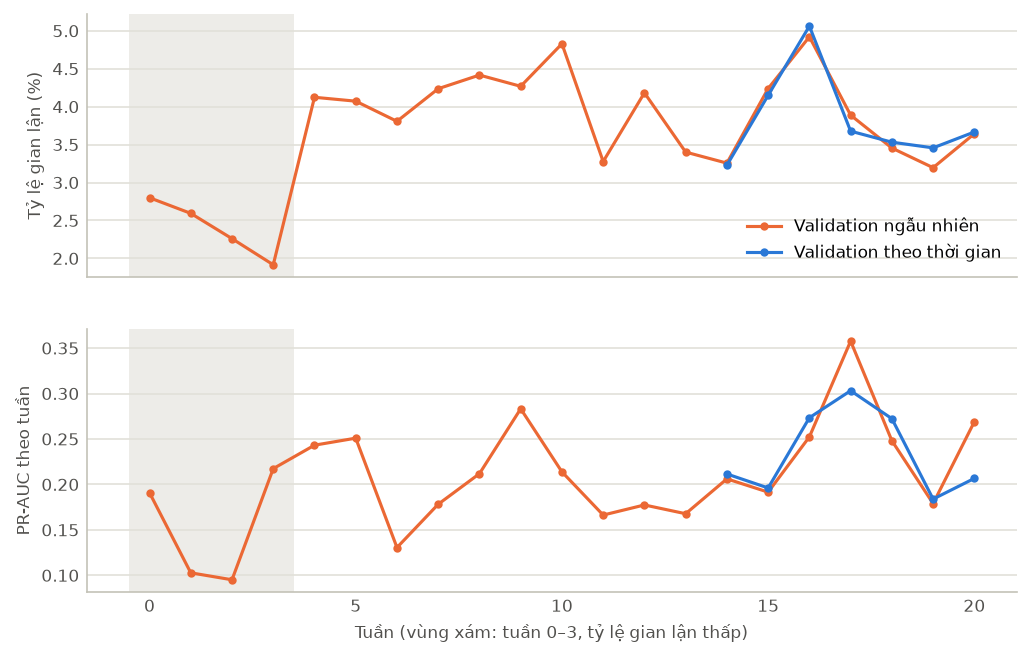
\includegraphics[width=0.92\linewidth]{figures/diag-weekly.png}
\caption{Tỷ lệ gian lận và PR-AUC theo tuần. Cam: mô hình huấn luyện ngẫu nhiên, chấm trên validation ngẫu nhiên (trải cả 6 tháng). Xanh: mô hình huấn luyện theo thời gian, chấm trên validation theo thời gian (tuần 14--20). Vùng xám: tuần 0--3.}
\end{figure}

\begin{keypoint}
\textbf{Kết luận.} (1) Hai cách chia đánh giá trên \emph{hai tập dòng khác nhau}; đổi tập đánh giá đổi PR-AUC khoảng 0,07, còn đổi cách huấn luyện chỉ đổi 0,001--0,012. (2) Tỷ lệ gian lận giải thích khoảng 0,012. (3) Tuần 0--3 có tỷ lệ gian lận 1,9--2,8\% và PR-AUC thấp (tuần 1--2 khoảng 0,10); bỏ chúng thì PR-AUC của validation ngẫu nhiên tăng từ 0,179 lên 0,212, tức khoảng một nửa mức chênh. Mốc ``tuần 0--3'' được chọn sau khi xem hình, nên đây là phân tích sau. (4) Khoảng 0,03 còn lại chưa giải thích. (5) Recall tại FPR 5\% gần như không đổi, nên không có bằng chứng mô hình kém đi. Chia ngẫu nhiên vẫn không chấp nhận được: trên cùng 29.223 dòng, mô hình huấn luyện ngẫu nhiên được lợi +0,0117 nhờ thấy giao dịch lân cận về thời gian.
\end{keypoint}

\subsubsection{Đặc trưng lịch sử thực thể}
Cùng dữ liệu, cách chia, lưới và Gradient Boosting với \code{gbm.yaml}; chỉ danh sách đặc trưng thay đổi.

\begin{table}[H]\centering\small
\caption{Gradient Boosting trên validation. ``Gốc'' là cấu hình đã chốt \code{run-f8807cb6f780}.}
\begin{tabularx}{\linewidth}{@{}Xccl@{}}
\toprule
Cấu hình & PR-AUC train & PR-AUC validation [95\% CI] & Lần chạy \\ \midrule
Gốc (20 đặc trưng) & 0,584 & 0,497 [0,483; 0,514] & \code{run-f8807cb6f780} \\
Lưới \code{max\_iter} đến 1.200 & 0,584 & 0,497 [0,483; 0,514] & \code{run-14499cc27f0a} \\
+ đếm tích luỹ, khoá \code{card1} & 0,689 & 0,497 [0,484; 0,513] & \code{run-0865527c0943} \\
+ đếm tích luỹ, khoá uid & 0,596 & 0,499 [0,484; 0,517] & \code{run-d15b7985126a} \\
+ đếm 24 giờ / 7 ngày, khoá \code{card1} & 0,690 & 0,5005 [0,487; 0,516] & \code{run-8f6422d09ac8} \\
+ đếm 24 giờ / 7 ngày, khoá uid & 0,594 & 0,4895 [0,476; 0,507] & \code{run-b7f7e893f155} \\
+ đếm 24 giờ / 7 ngày, khoá uid + \code{D1n} & 0,600 & 0,5085 [0,493; 0,523] & \code{run-f42906337c71} \\
+ thống kê tổng hợp, khoá uid & 0,609 & 0,4968 [0,483; 0,513] & \code{run-18a73d0c29f4} \\
+ thống kê tổng hợp, khoá uid + \code{D1n} & 0,607 & 0,4984 [0,483; 0,514] & \code{run-77d836c1ea94} \\ \midrule
Bỏ \code{C1}--\code{C14} (đối chứng) & 0,157 & 0,158 [0,149; 0,169] & \code{run-2d45949ed489} \\
Bỏ \code{C1}--\code{C14}, + lịch sử \code{card1} & 0,217 & 0,177 [0,167; 0,187] & \code{run-c5e7a212d3b8} \\
Bỏ \code{C1}--\code{C14}, + lịch sử uid & 0,226 & 0,174 [0,165; 0,185] & \code{run-8ecd86529b93} \\ \bottomrule
\end{tabularx}
\end{table}

\begin{table}[H]\centering\footnotesize\setlength{\tabcolsep}{3pt}
\caption{Bootstrap cặp so với gốc, 500 lần, trên cùng 118.108 dòng validation. In đậm: khoảng tin cậy loại trừ 0.}
\begin{tabular}{@{}lccc@{}}
\toprule
Biến thể & PR-AUC (dòng) & PR-AUC (cụm \code{card1}) & Recall @ FPR 5\% (cụm) \\ \midrule
Đếm, uid + \code{D1n} & \textbf{+0,0114} [+0,0054; +0,0168] & +0,0120 [$-$0,0026; +0,0249] & \textbf{+0,0218} [+0,0033; +0,0424] \\
Đếm, \code{card1} & +0,0035 [$-$0,0016; +0,0085] & +0,0036 [$-$0,0086; +0,0162] & +0,0025 [$-$0,0125; +0,0175] \\
Đếm, uid & \textbf{$-$0,0074} [$-$0,0118; $-$0,0030] & $-$0,0074 [$-$0,0191; +0,0035] & $-$0,0006 [$-$0,0169; +0,0150] \\
Tổng hợp, uid & $-$0,0002 [$-$0,0054; +0,0041] & $-$0,0002 [$-$0,0094; +0,0093] & +0,0041 [$-$0,0118; +0,0223] \\
Tổng hợp, uid + \code{D1n} & +0,0014 [$-$0,0053; +0,0081] & +0,0022 [$-$0,0117; +0,0173] & +0,0069 [$-$0,0074; +0,0235] \\ \bottomrule
\end{tabular}
\end{table}

\begin{keypoint}
\textbf{Kết luận.} (1) Các cột đếm \code{C1}--\code{C14} có sẵn trong dataset mang gần như toàn bộ tín hiệu theo thực thể: bỏ chúng thì PR-AUC rơi từ 0,497 xuống 0,158, và lịch sử tự dựng chỉ bù được khoảng 0,02. Đó là lý do thêm lịch sử không giúp. (2) Đếm tích luỹ tăng dần theo thời gian (số giữa của \code{card1} là 186 ở train, 629 ở validation), nhưng đổi sang đếm theo cửa sổ cũng không giúp. (3) Với khoá \code{card1}, PR-AUC train tăng mạnh (0,584 lên 0,69) mà validation đứng yên: mô hình học thuộc thẻ. (4) Khoá có \code{D1n} là biến thể tốt nhất, nhưng khi lấy mẫu theo cụm chỉ recall loại trừ 0, và sát 0; đây là biến thể tốt nhất trong 5 biến thể đã thử, chưa hiệu chỉnh nhiều lần so sánh. (5) Lưới rộng hơn không giúp, nên hạn chế ``tổ hợp nằm ở cạnh lưới'' của Stage E được gỡ bỏ. Cấu hình đã chốt và kết quả test 0,408 giữ nguyên.
\end{keypoint}

% ================================================================ 5
\section{Product 01 — Độ ổn định thanh toán}

\subsection{Dữ liệu giả lập (Stage C)}
\begin{table}[H]\centering
\caption{Hai bộ mô phỏng 7 ngày, 3 provider, 20 merchant, 150 payment/giờ.}
\begin{tabular}{@{}lcc@{}}
\toprule
Chỉ số & Tuning (\code{sim-485cacc9c858}) & Report (\code{sim-f6e6749ff0bf}) \\ \midrule
Payment / sự kiện & 25.573 / 30.050 & 25.151 / 29.340 \\
Payment có retry & 15,0\% & 14,3\% \\
Thành công ngay lần đầu & 77,1\% & 77,6\% \\
Thành công sau cùng & 89,9\% & 90,1\% \\
Độ trễ trung vị / p95 (ms) & 579 / 1.509 & 582 / 1.522 \\
Sự cố cài sẵn & 4 & 4 (có loại mới) \\ \bottomrule
\end{tabular}
\end{table}

\textbf{Vì sao 150 payment/giờ thay vì 30 như kế hoạch ban đầu.} Ở 30/giờ, mỗi provider chỉ có khoảng 2,5 attempt trong một khung 15 phút; tỷ lệ lỗi đo được dao động ngẫu nhiên khoảng $\pm 22$ điểm \%, lớn hơn chính tỷ lệ lỗi 15\%. Ở 150/giờ, dao động còn khoảng $\pm 10$ điểm \%. (Độ lệch chuẩn của một tỷ lệ là $\sqrt{p(1-p)/n}$.)

Mỗi bộ có thêm một sự cố \emph{yếu} (x1,5) để đo giới hạn phát hiện, vì sự cố mạnh (x3--x5) thì phương pháp nào cũng bắt được \cite{wu}. Cả hai bộ nạp vào PostgreSQL không có dòng bị từ chối.

\subsection{Kết quả detector (Stage D)}
Ngưỡng được chọn bằng lưới trên bộ tuning theo quy tắc viết trước: bắt nhiều bất thường nhất với tối đa 1 báo nhầm mỗi ngày; hoà thì chọn độ trễ ngắn hơn rồi ngưỡng cao hơn. Kết quả: D-A ngưỡng 7; D-B ngưỡng 8, gộp 2 khung. Cấu hình được commit (\code{e331ec1}, 14:27:02 UTC) \emph{trước} khi chạy bộ report (14:27:31 UTC).

\begin{table}[H]\centering
\caption{Tuning \code{det-3ddc26cff253}; report \code{det-08335c6af086} (một lần).}
\begin{tabular}{@{}lcc@{}}
\toprule
Detector & Tuning & Report \\ \midrule
D-B gộp cửa sổ & 3/4 sự cố, 0 báo nhầm/ngày & \textbf{2/4, 0 báo nhầm/ngày} \\
D-A z-score bền vững & 2/4, 1,0 báo nhầm/ngày & 0/4, 2,0 báo nhầm/ngày \\ \bottomrule
\end{tabular}
\end{table}

\begin{table}[H]\centering
\caption{Từng sự cố trên bộ report. Điểm cao nhất D-A / D-B; ngưỡng 7 / 8.}
\begin{tabular}{@{}llccc@{}}
\toprule
Sự cố & Đối tượng & Điểm & D-A & D-B \\ \midrule
Provider lỗi x3, 60 phút & \code{prov\_003} & 5,3 / 13,9 & Trượt & Bắt, sau 15 phút \\
Độ trễ tăng x2,5, 2 giờ & \code{prov\_002} & 6,0 / 12,7 & Trượt & Bắt, sau 30 phút \\
Mất lưu lượng QR x5, 2 giờ & QR & 3,6 / 6,6 & Trượt & \textbf{Trượt} \\
Provider lỗi x1,5, 2 giờ & \code{prov\_002} & 2,2 / 2,6 & Trượt & Trượt \\ \bottomrule
\end{tabular}
\end{table}

\begin{figure}[H]\centering
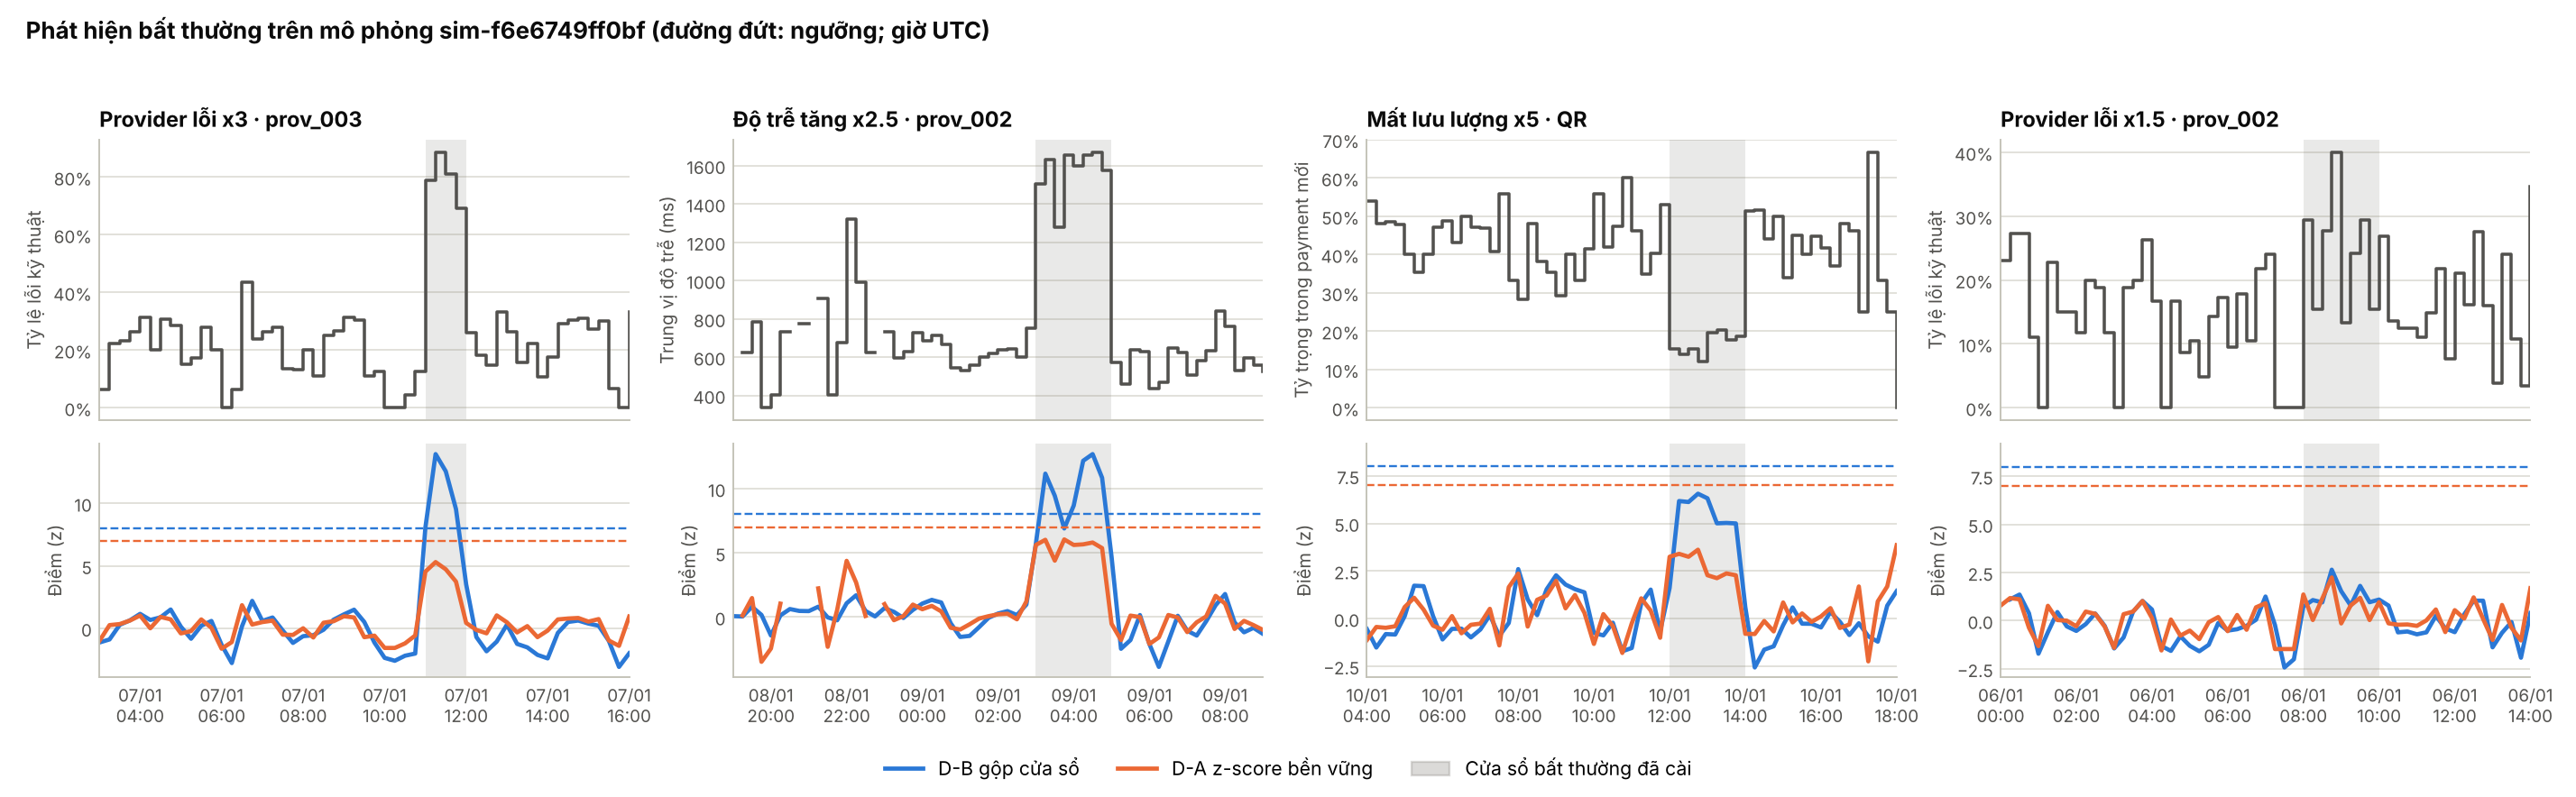
\includegraphics[width=\linewidth]{figures/stage-d-report.png}
\caption{Bộ report: KPI của đúng đối tượng quanh mỗi sự cố (trên) và điểm của hai detector (dưới). Vùng xám: cửa sổ sự cố cài sẵn.}
\end{figure}

\begin{keypoint}
\textbf{Đọc kết quả.}
\begin{itemize}
  \item \textbf{D-B tốt hơn D-A ở mọi mặt}, đúng lý do thiết kế: tính đến số attempt quan trọng hơn chọn ngưỡng khéo.
  \item \textbf{D-B trượt sự cố mất lưu lượng} dù nhìn bằng mắt rất rõ (tỷ trọng QR từ 44,0\% xuống 16,6\%): mỗi cửa sổ 30 phút chỉ có khoảng 110 payment mới, điểm đạt 6,6 dưới ngưỡng 8. Ngưỡng được chỉnh trên bộ tuning, nơi không có loại sự cố này. Đây chính là điều bộ report được thiết kế để lộ ra. Không chỉnh lại sau khi xem kết quả.
  \item \textbf{Sự cố x1,5 nằm dưới giới hạn phát hiện}: trên bộ report, tỷ lệ lỗi kỹ thuật của \code{prov\_002} chỉ tăng từ 16,2\% (24 giờ trước) lên 24,8\% (35/141 attempt); gộp cả 2 giờ được khoảng 2,8 độ lệch chuẩn, thấp xa ngưỡng 8 cần để không báo nhầm. Trên bộ tuning cũng vậy (\code{prov\_001}: 10,5\% lên 15,0\%).
  \item Mỗi bộ chỉ có 4 sự cố, nên đây là ví dụ minh hoạ, không phải tỷ lệ phát hiện.
\end{itemize}
\end{keypoint}

% ================================================================ 6
\section{Dashboard}
\code{make dashboard} tạo một trang HTML tĩnh từ kết quả các lần chạy: không thêm thư viện, mở được không cần mạng, đính được vào báo cáo (ADR 0007). Phần Product 01 có ô số tổng, bảng theo provider, biểu đồ theo giờ Việt Nam có tô vùng sự cố, danh sách sự cố (cảnh báo \code{ALL} trùng thời gian với cảnh báo một provider được gộp vào sự cố của provider đó, vì đó chỉ là tiếng vọng), và một bảng đối chiếu với sự cố cài sẵn được tách riêng (người vận hành thật không có nhãn). Biểu đồ ẩn các giờ có dưới 20 attempt, vì tỷ lệ tính trên vài attempt chủ yếu là nhiễu, đúng cái bẫy làm D-A báo nhầm.

Phần Product 02 có ô số PR-AUC test của từng mô hình, bảng mọi lần chạy (cột số đặc trưng ghi rõ biến thể, ví dụ ``24 (+4: uidd\_*)'' hay ``bỏ C1--C14''), bảng thí nghiệm rò rỉ, và hai mục mới: \emph{chia ngẫu nhiên và chia theo thời gian} (ma trận 2$\times$2 và biểu đồ theo tuần ở mục 4.5) và \emph{kiểm định cặp} (khoảng tin cậy loại trừ 0 được tô xanh). Trang có thanh điều hướng cố định ở đầu và tự đổi sang nền tối theo cài đặt của máy. Mục nào chưa có lần chạy thì ghi rõ lệnh cần chạy thay vì báo lỗi.

\begin{figure}[H]\centering
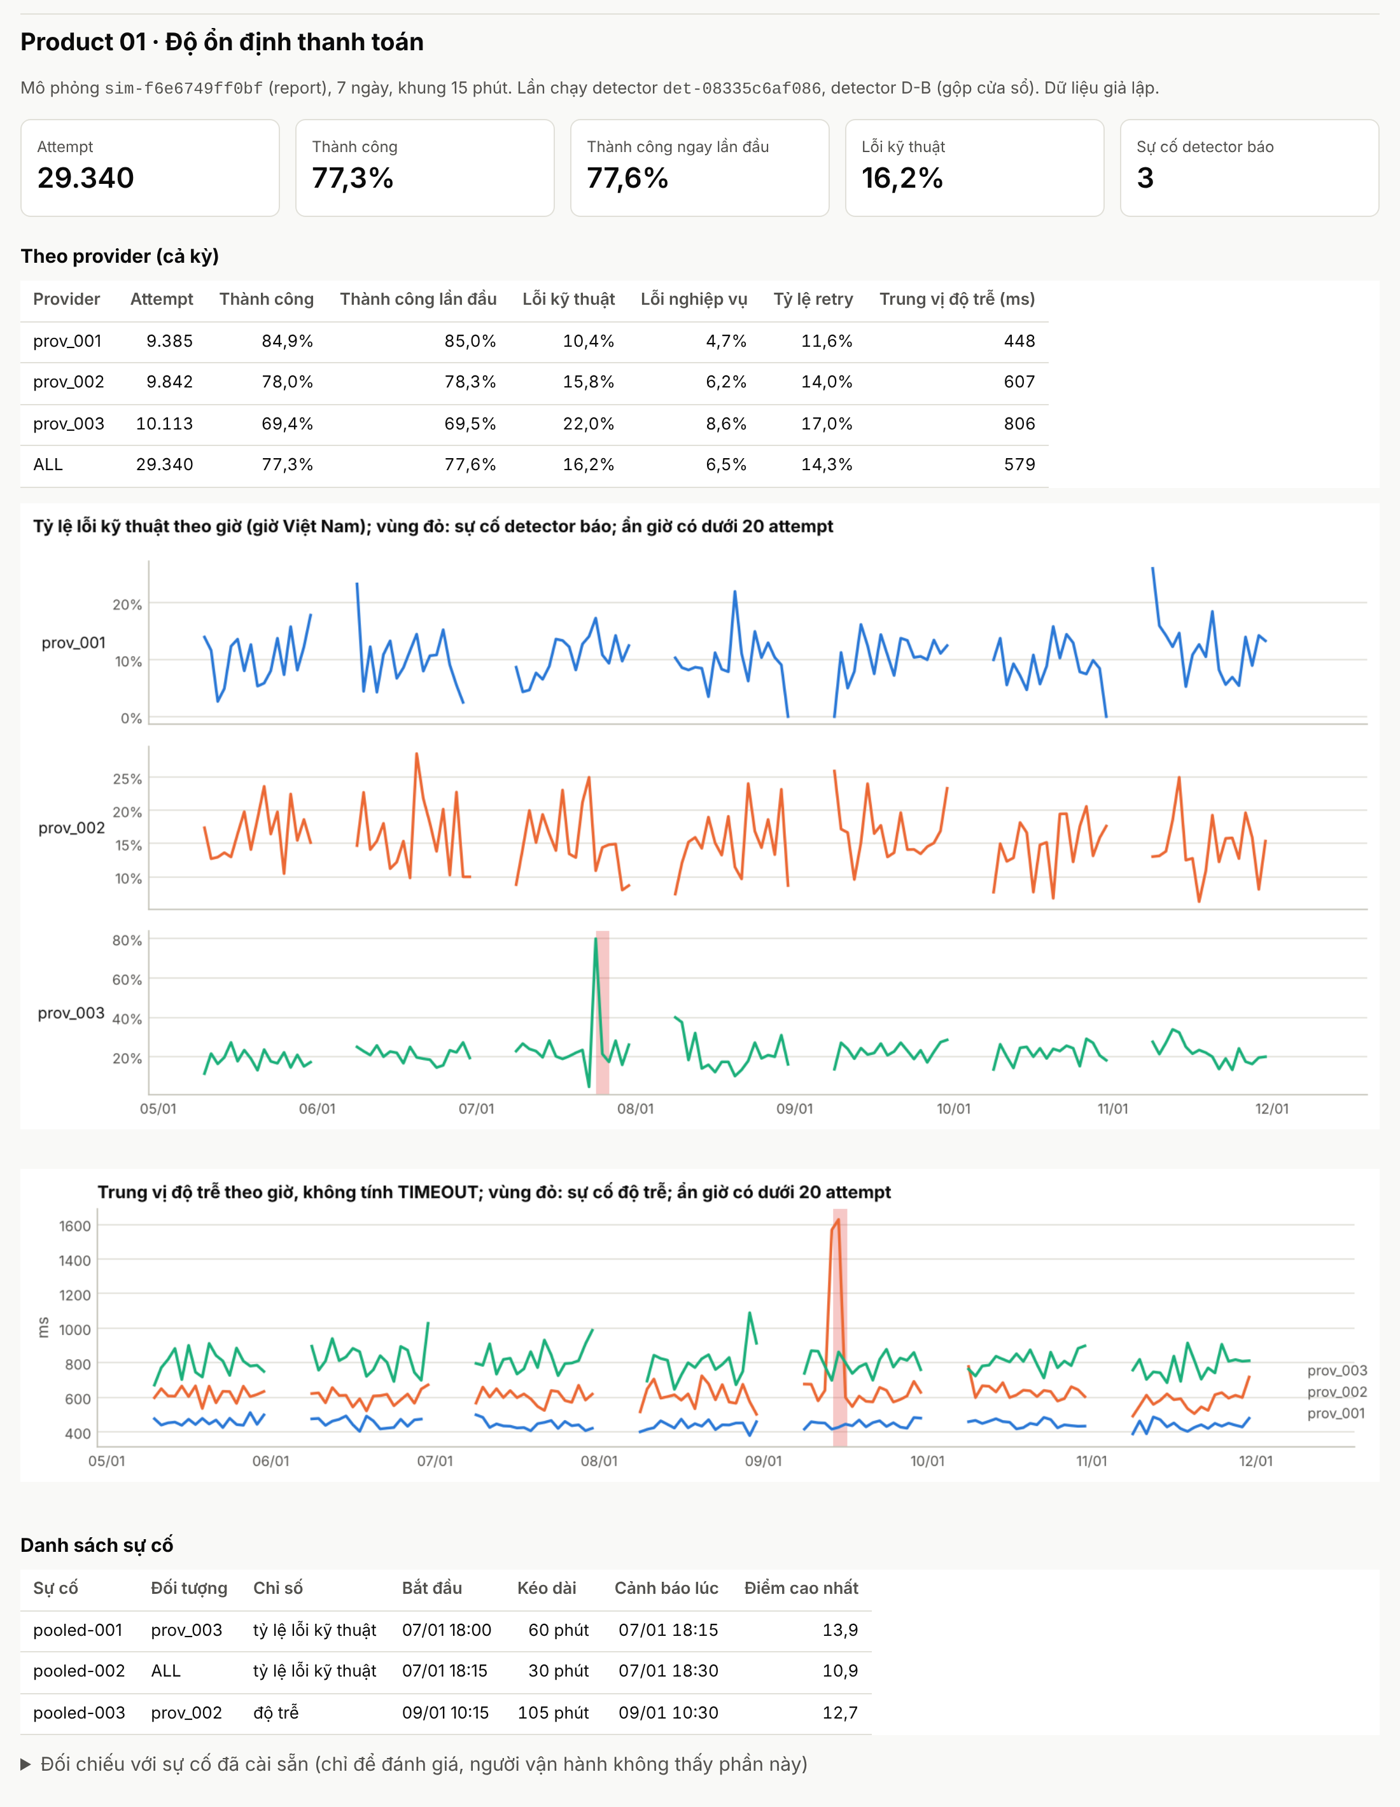
\includegraphics[width=0.82\linewidth]{figures/dashboard-product01.png}
\caption{Phần Product 01 của dashboard trên bộ report.}
\end{figure}

% ================================================================ 7
\section{Đánh giá trung thực và hạn chế}
\begin{itemize}
  \item \textbf{Test một lần}: mỗi cấu hình đã chốt chỉ mở tập test một lần; có sổ đăng ký chặn lần thứ hai. Danh sách cấu hình chạy test được đăng ký trước.
  \item \textbf{Dữ liệu Product 01 là giả lập}: mọi tham số do người làm đặt. Kết quả là ``kiểm chứng trên bất thường đã biết'', không phải hiệu năng thực tế.
  \item \textbf{IEEE-CIS}: nhãn lan theo tài khoản, cùng thẻ có thể xuất hiện ở cả train và test (ADR 0003). Chia theo thời gian không loại được hiện tượng này; thí nghiệm rò rỉ đo mức độ của nó.
  \item \textbf{Cỡ mẫu sự cố nhỏ}: 4 + 4 sự cố cài sẵn.
  \item \textbf{Giả định nhị thức của D-B} coi các attempt độc lập; retry của cùng payment không hoàn toàn độc lập.
  \item \textbf{Tái lập dữ liệu giả lập phụ thuộc phiên bản numpy}: \code{uv.lock} chọn numpy khác nhau cho Python 3.11 và 3.13; nên dùng cùng phiên bản khi muốn khớp từng byte. Mã lần chạy không chứa phiên bản thư viện: chạy lại thí nghiệm rò rỉ trên máy khác (Python 3.12) ra cùng mã \code{leak-827d929eaa73} nhưng lệch $\pm$0,001 ở 3 dòng; Gradient Boosting và hai baseline khớp hoàn toàn.
  \item \textbf{Hạ tầng}: PostgreSQL mới được kiểm chứng trên một bản cài tạm; đường \code{make up} trên WSL chưa thử.
  \item \textbf{Nguồn ý tưởng chưa xác minh}: khoá \code{D1n}, ý nghĩa của \code{C1}--\code{C14} và cách gộp thống kê lấy từ bài viết công khai thứ cấp của cuộc thi; đề tài chỉ dùng ý tưởng và kiểm chứng bằng thực nghiệm của mình.
  \item \textbf{Stage E}: còn khoảng 0,03 mức giảm PR-AUC khi chia ngẫu nhiên chưa giải thích, và cải thiện nhỏ của khoá có \code{D1n} chưa đủ ý nghĩa khi lấy mẫu theo cụm \code{card1}; mô hình chỉ dùng 20 đặc trưng (mục 4.3, 4.4).
\end{itemize}

% ================================================================ 8
\section{Hướng phát triển}
\begin{enumerate}
  \item \textbf{Kiểm chứng} phần còn lại của mức chênh khi chia ngẫu nhiên, và kiểm tra khoá có \code{D1n} trên giai đoạn dữ liệu mới (cần cấu hình mới và tập test mới).
  \item \textbf{API chấm điểm} (đã cắt khỏi 6 tuần): nhận một giao dịch, trả điểm rủi ro và lý do; chỉ hỗ trợ quyết định, không tự động chặn.
  \item \textbf{Ngưỡng riêng cho từng loại KPI}: chuỗi tỷ trọng ít nhiễu hơn chuỗi lỗi, nên một ngưỡng chung bỏ sót mất lưu lượng. Cần một bộ report mới để đánh giá trung thực.
  \item \textbf{Detector có mùa vụ}: so với cùng giờ các ngày trước (phân rã chuỗi thời gian \cite{fpp}), hoặc phương pháp dò thay đổi tích luỹ (CUSUM) để bắt sự cố yếu nhưng kéo dài.
  \item \textbf{Mô hình và đặc trưng}: LightGBM; đặc trưng theo thẻ chỉ dùng thông tin quá khứ; hiệu chỉnh xác suất; giải thích mô hình.
  \item \textbf{Nền tảng}: dbt thay SQL views khi số mô hình dữ liệu tăng; luồng sự kiện thời gian thực; theo dõi trôi dữ liệu.
  \item \textbf{Dữ liệu thật} khi có phê duyệt, cùng quy trình đánh giá đã xây.
\end{enumerate}

% ================================================================ 9
\section{Kết luận}
Trong 6 tuần, đề tài xây dựng nền tảng dùng chung (contract dữ liệu, quản lý dataset, quy tắc đánh giá, PostgreSQL) và hai sản phẩm có quy trình đánh giá giải thích được từng bước. Hai bài học rõ nhất: (1) với dữ liệu thay đổi theo thời gian, kết quả validation luôn lạc quan hơn test, nên phải giữ tập test cho một lần đo cuối; (2) với bài toán phát hiện bất thường, việc tính đến lượng dữ liệu phía sau mỗi con số quan trọng hơn việc chọn ngưỡng, và một bộ đánh giá độc lập có loại sự cố chưa gặp sẽ lộ ra những điểm mù mà bộ chỉnh ngưỡng không cho thấy.

% ================================================================ Phụ lục
\appendix
\section{Lệnh tái lập}
\begin{tabularx}{\linewidth}{@{}lX@{}}
\toprule
Lệnh & Việc \\ \midrule
\code{make setup}, \code{make lint test} & Cài môi trường, bật git hook; kiểm tra code \\
\code{make eda}, \code{make baseline} & EDA trên train; hai baseline trên validation \\
\code{make baseline-final} & Test một lần cho cấu hình đã chốt (chủ dự án) \\
\code{make simulate}, \code{make db-init}, \code{make ingest SIM=…} & Sinh và nạp dữ liệu giả lập \\
\code{make kpi SIM=…}, \code{make tune}, \code{make detect} & KPI, chỉnh ngưỡng, detector trên bộ tuning \\
\code{make detect-report} & Đánh giá một lần trên bộ report \\
\code{make leakage}, \code{make gbm}, \code{make gbm-final} & Stage E \\
\code{make gbm GBM\_CONFIG=…} & Một biến thể đặc trưng (cấu hình \code{draft}), chỉ validation \\
\code{python -m fraud\_risk.experiments.split\_diagnostics} & Chia ngẫu nhiên và chia theo thời gian (mục 4.5) \\
\code{python -m fraud\_risk.experiments.paired\_comparison} & Bootstrap cặp, theo dòng và theo cụm \code{card1} \\
\code{make dashboard} & Dashboard HTML \\ \bottomrule
\end{tabularx}

\section{Thuật ngữ}
\begin{tabularx}{\linewidth}{@{}lX@{}}
\toprule
Attempt & Một lần thử thanh toán; một payment có thể có nhiều attempt (retry) \\
Provider & Đối tác xử lý thanh toán \\
KPI & Chỉ số theo dõi, ở đây tính cho mỗi khung 15 phút \\
PR-AUC & Diện tích dưới đường precision--recall \\
FPR & Tỷ lệ giao dịch hợp lệ bị báo nhầm \\
Rò rỉ dữ liệu & Mô hình dùng thông tin không có lúc dự đoán thật \\
Concept drift & Quan hệ giữa dữ liệu và nhãn thay đổi theo thời gian \\
ADR & Tài liệu ghi một quyết định kiến trúc và lý do \\
\code{frozen} & Cấu hình đã chốt; chỉ chủ dự án đặt \\ \bottomrule
\end{tabularx}

% ================================================================ Tài liệu
\begin{thebibliography}{99}\small
\bibitem{saito} T. Saito, M. Rehmsmeier. The Precision-Recall Plot Is More Informative than the ROC Plot When Evaluating Binary Classifiers on Imbalanced Datasets. \emph{PLOS ONE} 10(3), 2015.
\bibitem{jesus} S. Jesus et al. Turning the Tables: Biased, Imbalanced, Dynamic Tabular Datasets for ML Evaluation. NeurIPS 2022 Datasets and Benchmarks, arXiv:2211.13358.
\bibitem{kaufman} S. Kaufman, S. Rosset, C. Perlich, O. Stitelman. Leakage in Data Mining: Formulation, Detection, and Avoidance. \emph{ACM TKDD} 6(4), 2012.
\bibitem{kapoor} S. Kapoor, A. Narayanan. Leakage and the Reproducibility Crisis in Machine-Learning-Based Science. \emph{Patterns} 4(9), 2023.
\bibitem{gama} J. Gama, I. Žliobaitė, A. Bifet, M. Pechenizkiy, A. Bouchachia. A Survey on Concept Drift Adaptation. \emph{ACM Computing Surveys} 46(4), 2014.
\bibitem{grinsztajn} L. Grinsztajn, E. Oyallon, G. Varoquaux. Why Do Tree-Based Models Still Outperform Deep Learning on Typical Tabular Data? NeurIPS 2022 Datasets and Benchmarks.
\bibitem{handbook} Y.-A. Le Borgne, W. Siblini, B. Lebichot, G. Bontempi. \emph{Reproducible Machine Learning for Credit Card Fraud Detection — Practical Handbook}. ULB, 2022.
\bibitem{dalpozzolo} A. Dal Pozzolo et al. Credit Card Fraud Detection: A Realistic Modeling and a Novel Learning Strategy. \emph{IEEE TNNLS} 29(8), 2018.
\bibitem{sre} B. Beyer, C. Jones, J. Petoff, N. R. Murphy (eds.). \emph{Site Reliability Engineering}. O'Reilly, 2016.
\bibitem{fpp} R. J. Hyndman, G. Athanasopoulos. \emph{Forecasting: Principles and Practice}, 3rd ed. OTexts, 2021.
\bibitem{wu} R. Wu, E. Keogh. Current Time Series Anomaly Detection Benchmarks Are Flawed and Are Creating the Illusion of Progress. \emph{IEEE TKDE}, 2021.
\bibitem{lavin} A. Lavin, S. Ahmad. Evaluating Real-time Anomaly Detection Algorithms — the Numenta Anomaly Benchmark. ICMLA 2015.
\bibitem{chandola} V. Chandola, A. Banerjee, V. Kumar. Anomaly Detection: A Survey. \emph{ACM Computing Surveys} 41(3), 2009.
\bibitem{jsonschema} JSON Schema Specification, bản 2020-12. \url{https://json-schema.org/specification}.
\bibitem{kleppmann} M. Kleppmann. \emph{Designing Data-Intensive Applications}. O'Reilly, 2017.
\bibitem{paysim} E. Lopez-Rojas, A. Elmir, S. Axelsson. PaySim: A Financial Mobile Money Simulator for Fraud Detection. EMSS 2016.
\bibitem{nygard} M. Nygard. Documenting Architecture Decisions, 2011.
\bibitem{ieee} IEEE-CIS Fraud Detection, Kaggle. \url{https://www.kaggle.com/c/ieee-fraud-detection}. Chỉ dùng cho nghiên cứu, theo điều khoản cuộc thi.
\end{thebibliography}

\end{document}
